\documentclass[runningheads]{llncs}

% ==============================================================================
% Gói hỗ trợ ngôn ngữ và Định dạng
% ==============================================================================
\usepackage[utf8]{inputenc}
\usepackage[vietnamese,english]{babel}
\usepackage[T5,T1]{fontenc}

% Nhúng các macro, thư viện toán học và thuật toán
% ==============================================================================
% Mathematical Notation and Custom Macros for OrthoStyle Paper
% ==============================================================================

% Springer LNCS and amsmath compatibility for \vec
\let\accentvec\vec
\usepackage{amsmath,amssymb,amsfonts}
\let\spvec\vec
\let\vec\accentvec
\usepackage{bm}
\usepackage{xspace}
\usepackage{booktabs}
\usepackage{multirow}
\usepackage{graphicx}
\usepackage{hyperref}
\usepackage{url}
\usepackage{xcolor}
\usepackage{algorithm}
\usepackage{algorithmic}

% Method Name
\newcommand{\method}{\textsc{OrthoStyle}\xspace}
\newcommand{\ours}{\textsc{OrthoStyle}\xspace}

% Math Vectors and Matrices
\newcommand{\bx}{\mathbf{x}}
\newcommand{\bz}{\mathbf{z}}
\newcommand{\by}{\mathbf{y}}
\newcommand{\bc}{\mathbf{c}}
\newcommand{\bs}{\mathbf{s}}
\newcommand{\bg}{\mathbf{g}}
\newcommand{\bv}{\mathbf{v}}
\newcommand{\bu}{\mathbf{u}}
\newcommand{\bk}{\mathbf{k}}
\newcommand{\bq}{\mathbf{q}}
\newcommand{\beps}{\boldsymbol{\epsilon}}
\newcommand{\btheta}{\boldsymbol{\theta}}
\newcommand{\bmu}{\boldsymbol{\mu}}
\newcommand{\bsigma}{\boldsymbol{\sigma}}

% Subspaces and Operators
\newcommand{\Vsub}{\mathcal{V}_{\text{sub}}}
\newcommand{\Vortho}{\mathcal{V}_{\text{sub}}^\perp}
\newcommand{\Proj}{\text{Proj}}
\newcommand{\norm}[1]{\left\lVert#1\right\rVert}
\newcommand{\inner}[2]{\left\langle #1, #2 \right\rangle}
\newcommand{\E}{\mathbb{E}}
\newcommand{\R}{\mathbb{R}}
\newcommand{\Loss}{\mathcal{L}}

% Attention Variables
\newcommand{\xtxt}{\mathbf{x}_{\text{txt}}}
\newcommand{\xsub}{\mathbf{x}_{\text{sub}}}
\newcommand{\xstyle}{\mathbf{x}_{\text{style}}}
\newcommand{\xsubstyle}{\mathbf{x}_{\text{sub\_style}}}
\newcommand{\xstyleortho}{\mathbf{x}_{\text{style}}^\perp}
\newcommand{\xsubstyleortho}{\mathbf{x}_{\text{sub\_style}}^\perp}
\newcommand{\wtxt}{w_{\text{txt}}}
\newcommand{\wsub}{w_{\text{sub}}}
\newcommand{\wstyle}{w_{\text{style}}}
\newcommand{\wsubstyle}{w_{\text{sub\_style}}}

% Formatting helpers
\newcommand{\best}[1]{\textbf{#1}}
\newcommand{\second}[1]{\underline{#1}}
\newcommand{\fixme}[1]{\textcolor{red}{[FIXME: #1]}}
\newcommand{\todo}[1]{\textcolor{blue}{[TODO: #1]}}


\title{\method: Manifold-Preserving Training-Free Style Transfer via Score-Orthogonal Guidance}

\titlerunning{\method: Manifold-Preserving Training-Free Style Transfer}

\author{Nhat Minh Nguyen\inst{1,2} \and
Quang Dang Pham\inst{1,2}\and
Phuc Thien Vo\inst{1,2}\and
Loc Phuc Dang\inst{1,2}\and
Khoan Duc Le\inst{1,2}\thanks{Corresponding author}}

\authorrunning{N.Nhat et al.}

\institute{Faculty of Information Technology, University of Science, Ho Chi Minh City, Vietnam \\
\email{\{2512021580, 2512022643, 2512022237, 2512020320\}@student.hcmus.edu.vn}\\
\email{ldkhoan@fit.hcmus.edu.vn}
\and
Vietnam National University, Ho Chi Minh City, Vietnam
}

\begin{document}

\selectlanguage{vietnamese}

\maketitle

% ==============================================================================
% Tóm tắt (Abstract)
% ==============================================================================
\begin{abstract}
Truyền tải phong cách dựa trên hình ảnh tham chiếu (reference-based style transfer) với các mô hình khuếch tán hướng tới mục tiêu tổng hợp chất liệu nghệ thuật trong khi bảo toàn cấu trúc hình học và ngữ nghĩa của ảnh mục tiêu. Tuy nhiên, các phương pháp không cần huấn luyện (training-free) đối mặt với sự đánh đổi giữa độ trung thực phong cách và bảo toàn nội dung: việc áp đặt phong cách quá mạnh có thể làm biến dạng cấu trúc và gây rò rỉ nội dung (content leakage), trong khi truyền tải thận trọng thường dẫn đến hiện tượng thiếu hụt phong cách hóa (under-stylization). Chúng tôi giới thiệu \method, một khung làm việc training-free giải quyết sự đánh đổi này mà không cần fine-tuning mạng hay sử dụng kỹ thuật DDIM inversion. \method bao gồm ba thành phần: Semantic Gating để bảo toàn các đặc trưng hình học và ngữ nghĩa; Score-Orthogonal DINO Guidance nhằm chiếu gradient phong cách trực giao với hướng vector score khuếch tán, bảo toàn quỹ đạo lấy mẫu luôn bám sát đa tạp dữ liệu; và Bộ điều khiển bước sớm (Early Step Controller) áp dụng AdaIN-based clean-latent pushforward để cố định màu sắc và bố cục trước khi tinh chỉnh phong cách chi tiết. Các so sánh định lượng và định tính toàn diện với cả các baseline dựa trên điều khiển tối ưu (OC-based) lẫn các phương pháp phong cách hóa tiêu biểu chứng minh \method đạt được sự cân bằng tối ưu giữa độ trung thực phong cách và bảo toàn nội dung trong khi duy trì tính nhất quán cấu trúc. Đáng chú ý nhất, phương pháp của chúng tôi vượt trội hoàn toàn so với mô hình baseline sử dụng chung kiến trúc nền tảng Stable Cascade.

\keywords{Style Transfer \and Training-free \and Score-Orthogonal Guidance \and Diffusion Models.}
\end{abstract}

% ==============================================================================
% Phần 1: Giới thiệu (Introduction)
% ==============================================================================
\section{Giới thiệu}
\label{sec:intro}

Các mô hình khuếch tán Text-to-Image (T2I)~\cite{sd,wuerstchen,ddpm} đã tạo ra một bước nhảy vọt trong lĩnh vực tổng hợp thị giác số, chứng minh năng lực phi thường trong việc tạo ra các hình ảnh giàu tính thẩm mỹ và độ trung thực cao từ các mô tả văn bản tự nhiên. Những mô hình nền tảng này ngày càng được ứng dụng sâu rộng trong các ngành công nghiệp sáng tạo, từ thiết kế nghệ thuật số, thiết kế nhân vật trong trò chơi điện tử, cá nhân hóa đối tượng thị giác cho đến chỉnh sửa ảnh định hướng văn bản~\cite{prompt2prompt,instructpix2pix}. Trong các quy trình sáng tạo này, các nhà thiết kế luôn đòi hỏi quyền kiểm soát độc lập và chuẩn xác cả về mặt cấu trúc nội dung ngữ nghĩa lẫn phong cách thị giác nghệ thuật. Mặc dù cấu trúc nội dung của một hoạt cảnh (ví dụ: "một chiếc đồng hồ cổ điển đặt trên bàn gỗ" hoặc "một chú mèo đang ngồi") có thể được đặc tả tường minh thông qua văn bản, nhưng việc truyền đạt phong cách nghệ thuật đặc trưng của một nghệ sĩ---được định hình bởi các lớp cọ dày (impasto), độ loang sắc tố tinh vi, các kết cấu hình học phi Euclid, và các đặc tính vật lý đặc thù của chất liệu (như sơn dầu, kính màu ghép, tranh khắc gỗ truyền thống, origami, hay phong cách viễn tưởng cyberpunk rực rỡ neon)---lại là những khái niệm trừu tượng, phi ngôn ngữ và vô cùng phức tạp. Do đó, việc biểu đạt những sắc thái phong cách tinh tế này chỉ bằng các mô tả văn bản thông thường gặp phải rào cản nghiêm trọng về giới hạn từ vựng và sự mơ hồ ngữ nghĩa. Thực tế này đã thúc đẩy sự ra đời của hướng nghiên cứu cá nhân hóa phong cách thông qua hình ảnh tham chiếu (exemplar-based visual style personalization) như một nhánh phát triển tất yếu trong thị giác máy tính tạo sinh~\cite{stylealigned,instantstyle,rout2025rbmodulation}.

% ==============================================================================
% Teaser Figure: Ma trận Định tính Tổng thể (Content x Style)
% ==============================================================================
\begin{figure*}[t]
\centering
\includegraphics[width=\textwidth]{figs/qualitative_matrix_teaser.png}
\caption{\textbf{Ma Trận Phong Cách Hóa Định Tính của \method Trên Đa Dạng Danh Mục Nội Dung và Phong Cách Nghệ Thuật.} 
Các hàng tương ứng với các đối tượng content đại diện qua nhiều miền ngữ nghĩa (động vật, đồ vật sinh hoạt, trang phục); các cột tương ứng với các phong cách nghệ thuật đa dạng (sơn dầu, tranh ghép mosaic, khắc gỗ, cyberpunk phát sáng, và kết xuất 3D). Mọi kết quả đều được sinh ra dưới cơ chế suy luận không cần prompt (null-prompt inference, tương tự như RB-Modulation~\cite{rout2025rbmodulation}), thể hiện khả năng bảo toàn chuẩn xác hình học và tư thế đối tượng trong khi truyền tải trọn vẹn nét cọ và chất liệu nghệ thuật mà không bị rò rỉ ngữ nghĩa.}
\label{fig:teaser_matrix}
\end{figure*}

Nhằm cá nhân hóa các mô hình diffusion đã huấn luyện trước cho một phong cách nghệ thuật cụ thể, các nghiên cứu hiện nay chủ yếu phát triển theo hai trường phái chính: (1) tối ưu hóa dựa trên fine-tuning và (2) điều biến suy luận không cần huấn luyện (training-free inference modulation). Các phương pháp fine-tuning---tiêu biểu như DreamBooth~\cite{dreambooth}, Custom Diffusion, LoRA~\cite{lora}, ZipLoRA~\cite{ziplora}, StyleDrop~\cite{styledrop}, và B-LoRA~\cite{b-lora}---tối ưu hóa các vector nhúng từ khóa (text embeddings), các ma trận chiếu cross-attention, hoặc các trọng số thích ứng hạng thấp (low-rank adapters) thông qua hàm mục tiêu khử nhiễu khuếch tán. Khi được huấn luyện trên một tập hợp gồm nhiều hình ảnh tham chiếu cùng phong cách (thường từ 4 đến 10 ảnh được chọn lọc cẩn thận), các phương pháp này có khả năng nắm bắt phong cách tương đối tốt. Tuy nhiên, chúng bộc lộ ba điểm nghẽn thực tiễn mang tính sống còn:
(i) việc thu thập nhiều tác phẩm nghệ thuật chất lượng cao có cùng một phong cách đồng nhất là cực kỳ khó khăn hoặc bất khả thi, đặc biệt đối với các kiệt tác hội họa lịch sử độc bản hoặc các bản vẽ thiết kế kỹ thuật số đơn lẻ;
(ii) việc thực thi chu trình lan truyền ngược gradient cho mỗi phong cách mới tiêu tốn tài nguyên và thời gian tính toán quá lớn (yêu cầu vài phút tính toán trên GPU cho mỗi phong cách); và
(iii) quan trọng nhất, khi chỉ được cung cấp một \textit{hình ảnh tham chiếu duy nhất}, các kỹ thuật fine-tuning gặp phải hiện tượng ghi nhớ ngữ nghĩa tai hại và quá khớp (catastrophic semantic memorization / overfitting)---mô hình vô tình ghi nhớ và tái tạo lại chính các vật thể cụ thể xuất hiện trong bức tranh mẫu (ví dụ: vẽ lại nguyên vẹn chân dung một con người hay tòa nhà) thay vì trích xuất bản chất phong cách nghệ thuật trừu tượng.

Để triệt tiêu hoàn toàn chi phí tính toán nặng nề và sự phụ thuộc vào dữ liệu nhiều ảnh của phương pháp fine-tuning, các nghiên cứu gần đây chuyển hướng sang phương pháp training-free, can thiệp trực tiếp vào các vector keys, values và các bản đồ đặc trưng bên trong các tầng attention của mô hình khuếch tán tại thời điểm suy luận~\cite{stylealigned,instantstyle,styleid,diffstyler,freestyle}. Tuy vậy, các khung làm việc training-free hiện nay vẫn vấp phải những thách thức nan giải trong việc tách rời phong cách khỏi nội dung ngữ nghĩa và chuyển giao phong cách mà không làm biến dạng cấu trúc:
- *Các phương pháp dựa trên đảo ngược khuếch tán (StyleAligned~\cite{stylealigned}, Swapping Self-Attention)*: Đồng bộ hóa phong cách giữa các ảnh bằng cách chia sẻ keys và values trong self-attention. Tuy nhiên, các kỹ thuật này phụ thuộc vào quá trình DDIM inversion tất định~\cite{DDIM} để lưu trữ đặc trưng tham chiếu, vốn dĩ làm suy giảm nghiêm trọng các chi tiết vân bề mặt tần số cao và tích lũy sai số rời rạc hóa; hơn nữa, chúng đòi hỏi hai tiến trình khuếch tán ngược chạy song song, làm tăng gấp đôi mức tiêu thụ bộ nhớ VRAM và thời gian suy luận.
- *Các phương pháp tiêm đặc trưng qua Cross-Attention (InstantStyle~\cite{instantstyle})*: Tiêm các đặc trưng thị giác từ ảnh style vào một tập con các tầng cross-attention được chọn lọc heuristic bên trong mô hình IP-Adapter~\cite{ipadapter} đã huấn luyện sẵn. Mặc dù vậy, việc xác định thủ công các tầng tiêm đặc trưng mang tính thực nghiệm thiếu tính tổng quát hóa trên các kiến trúc mô hình khác nhau. Trầm trọng hơn, phép cộng tuyến tính các vector đặc trưng trực tiếp gây ra hiện tượng \textbf{rò rỉ nội dung (content leakage)} nghiêm trọng---vô tình tổng hợp các vật thể ngoại lai từ ảnh style vào hình ảnh đích (ví dụ: sinh thêm rồng hoặc lâu đài khi người dùng chỉ mong muốn hiệu ứng kim loại vàng tan chảy). Để ngăn chặn sự sụp đổ hình học, InstantStyle bắt buộc phải phụ thuộc vào mạng ControlNet bổ trợ~\cite{controlNet}, điều này gò bó quá trình tạo ảnh vào các khung bố cục cứng nhắc và bóp nghẹt tính đa dạng sáng tạo.
- *Điều khiển tối ưu ngẫu nhiên (RB-Modulation~\cite{rout2025rbmodulation})*: RB-Modulation đề xuất khung điều khiển tối ưu ngẫu nhiên với hàm chi phí biên (terminal style cost), loại bỏ sự phụ thuộc vào các mạng adapter bên ngoài. Tuy nhiên, để ngăn chặn hiện tượng rò rỉ nội dung, RB-Modulation bắt buộc phải áp dụng phép \textbf{gộp trung bình không gian cực đoan (mean-pooling)} ($\bar{\mathbf{t}}_{\text{style}} = \frac{1}{L} \sum_{j=1}^L \mathbf{t}_{\text{style}}^{(j)}$) trên toàn bộ các style token tham chiếu. Mặc dù việc ép tất cả các token về một vector trung bình tĩnh giúp triệt tiêu ngữ nghĩa vật thể, \textbf{nó triệt tiêu toàn bộ phương sai không gian của các token phong cách}, dẫn đến hiện tượng \textbf{thiếu hụt phong cách hóa trầm trọng (under-stylization)}, các nét cọ nghệ thuật bị làm phẳng bẹt, chất liệu nhạt nhòa và chỉ mang tính chất đổi màu bề mặt. Thêm vào đó, việc cập nhật gradient không ràng buộc đẩy quỹ đạo lấy mẫu lệch khỏi đa tạp dữ liệu thực, và việc phụ thuộc vào metric CSD giám sát thường gây sụp đổ miền biểu diễn khi gặp các chất liệu nghệ thuật phi thực tế phức tạp. Do đó, các phương pháp hiện tại rơi vào tình thế phân cực nhức nhối: hoặc sụp đổ nội dung và rò rỉ vật thể nặng nề (như InstantStyle, DiffuseIT~\cite{diffuseIT}), hoặc thiếu hụt phong cách và suy thoái chất liệu (như RB-Modulation, ITOC).

Để giải quyết dứt điểm sự đánh đổi này, chúng tôi đề xuất \textbf{\method}, một khung làm việc training-free toàn diện được xây dựng trên kiến trúc mô hình khuếch tán phân tầng (Stable Cascade~\cite{wuerstchen}). \method thiết lập một đường biên tối ưu Pareto mới mà không cần fine-tuning mạng, không cần DDIM inversion, và không phụ thuộc vào text prompt. Thay vì thỏa hiệp giữa độ bảo toàn nội dung và cường độ phong cách, \method dung hòa cả hai thông qua ba cơ chế toán học bổ trợ:
\begin{itemize}
    \item \textbf{Blended Style Tokens với Phép Chiếu Trực Giao Không Gian Triệt Tiêu (Null-Space)}: Chúng tôi đề xuất toán tử pha trộn mềm ($\alpha_s = 0.85$) nhằm bảo toàn phương sai chất liệu tần số cao đồng thời làm mượt các dị thường ngữ nghĩa cục bộ. Bằng việc chiếu trực giao các style query lên không gian bù trực giao (null space) của biểu diễn nội dung $\Vortho$ ngay trong các tầng cross-attention, \method triệt tiêu hoàn toàn sự can nhiễu đặc trưng, loại bỏ dứt điểm rò rỉ vật thể trong khi khôi phục trọn vẹn chất liệu nét cọ sống động.
    \item \textbf{Điều hướng DINO Trực Giao với Score Khuếch Tán (Score-Orthogonal DINO Guidance)}: Chúng tôi xây dựng hàm loss điều hướng biên trong không gian đặc trưng của mạng Vision Transformer tự giám sát (DINO-ViT-S/16)~\cite{dino}. Do DINO được huấn luyện tự chắt lọc không cần nhãn phân loại văn bản, các biểu diễn của nó bắt trọn sự đồng xuất hiện kết cấu không gian trung cấp, tính liên tục của bề mặt và hướng nét cọ mà không bị thiên lệch ngữ nghĩa. Bằng cách chiếu gradient điều hướng lên null space của vector score khuếch tán, \method bảo toàn trọn vẹn đa tạp dữ liệu, dập tắt hiện tượng trôi dạt khỏi phân phối và triệt tiêu hoàn toàn các dị tật bão hòa màu.
    \item \textbf{Bộ Điều Khiển Bước Sớm AdaIN Pushforward (Early-Step Controller)}: Dựa trên nguyên lý đánh đổi nhiễu ngẫu nhiên được xác lập trong SDEdit~\cite{sdedit}---trong đó các bước khuếch tán sớm quyết định cấu trúc không gian tổng thể còn các bước muộn quyết định chất liệu chi tiết---\method áp dụng chuẩn hóa thích ứng thể hiện (AdaIN) trực tiếp lên clean latent dự đoán $\bx_0$ tại các bước lấy mẫu ban đầu. Cơ chế này nhanh chóng định hình phân phối màu sắc và độ tương phản vĩ mô mà không làm nhiễu loạn quá trình tổng hợp nét vẽ ở giai đoạn sau.
\end{itemize}

Các đóng góp chính của bài báo được tóm tắt như sau:
\begin{enumerate}
    \item Chúng tôi đề xuất \textbf{\method}, một khung làm việc cắm-và-chạy (plug-and-play), không cần huấn luyện cho bài toán truyền tải phong cách dựa trên hình ảnh tham chiếu, thiết lập đường biên tối ưu Pareto vượt trội mà không cần fine-tuning, DDIM inversion hay kỹ thuật prompt engineering phức tạp.
    \item Chúng tôi giới thiệu cơ chế \textbf{Blended Style Tokens kết hợp Phép Chiếu Trực Giao Null-Space và Bù Năng Lượng}, giải quyết triệt để sự đánh đổi giữa hiện tượng rò rỉ nội dung của InstantStyle và sự sụp đổ chất liệu của phép mean pooling trong RB-Modulation.
    \item Chúng tôi xây dựng cơ chế \textbf{Score-Orthogonal DINO Latent Guidance} với chứng minh toán học chặt chẽ về tính bảo toàn đa tạp, tận dụng các biểu diễn patch tự giám sát của DINO như một bộ hòa hợp chất liệu nhằm định hướng các nét vẽ nghệ thuật tinh tế mà không gây thiên lệch ngữ nghĩa vật thể.
    \item Chúng tôi thiết kế \textbf{Bộ Điều Khiển Bước Sớm AdaIN Pushforward} dựa trên nguyên lý đánh đổi ngẫu nhiên SDEdit kết hợp với tiền xử lý tách biên Canny ngữ nghĩa, chứng minh tính ưu việt tuyệt đối cả về mặt định tính lẫn định lượng so với sáu phương pháp SOTA trên bộ dữ liệu chuẩn 225 cặp ảnh SOICT-Data.
\end{enumerate}

% ==============================================================================
% Phần 2: Công trình Liên quan (Related Work)
% ==============================================================================
\section{Công trình Liên quan}
\label{sec:related}

\subsection{Cá nhân hóa Mô hình Khuếch tán Text-to-Image}
Các mô hình khuếch tán Text-to-Image (T2I)~\cite{ddpm,sd,wuerstchen} đã trở thành các công cụ tạo sinh tiên tiến nhất hiện nay, mở rộng ranh giới về độ chân thực thị giác, tính kết hợp và khả năng tuân thủ văn bản. Khả năng tổng hợp dữ liệu chiều cao thông qua việc học trường drift đảo ngược của phương trình vi phân ngẫu nhiên thuận~\cite{songscore} đã mở ra vô số ứng dụng sáng tạo. Bên cạnh việc sinh ảnh tự do, các nghiên cứu về cá nhân hóa mô hình khuếch tán đã mở rộng trên nhiều phương diện: chỉnh sửa ảnh cục bộ định hướng văn bản~\cite{prompt2prompt,instructpix2pix}, giải quyết các bài toán nghịch đảo tuyến tính và phi tuyến~\cite{dps}, sinh ảnh định hướng khái niệm và bảo toàn danh tính chủ thể~\cite{dreambooth,lora}, cũng như tổng hợp ảnh theo phong cách hóa~\cite{stylealigned,instantstyle,rout2025rbmodulation}.

Trong bài toán cá nhân hóa dựa trên ảnh mẫu (exemplar-based personalization), mục tiêu cốt lõi là điều khiển quá trình tạo sinh bằng các gợi ý thị giác trực tiếp từ ảnh tham chiếu thay vì phụ thuộc hoàn toàn vào văn bản. Để điều chỉnh một mô hình diffusion nền tảng cho một đối tượng hoặc phong cách mục tiêu, các công trình hiện tại phân chia thành hai phương pháp luận chủ đạo: (1) tinh chỉnh tối ưu hóa (fine-tuning toàn bộ mô hình hoặc thích ứng tham số hiệu quả) và (2) điều biến trực tiếp trong quá trình suy luận (training-free). Trong khi fine-tuning làm biến đổi các trọng số của mạng, các phương pháp training-free tác động động lên các kích hoạt đặc trưng nội bộ hoặc các quỹ đạo lấy mẫu của mô hình đã bị đóng băng.

\subsection{Fine-Tuning Mô hình Khuếch tán cho Phong cách Nghệ thuật}
Các phương pháp fine-tuning tối ưu hóa các tham số mạng để căn chỉnh các biểu diễn nội tại khớp với hình ảnh tham chiếu. Kỹ thuật fine-tuning toàn phần như DreamBooth~\cite{dreambooth} tối ưu hóa toàn bộ mạng U-Net cùng với các token văn bản định danh, mang lại năng lực biểu đạt cao nhưng đòi hỏi chi phí lưu trữ và bộ nhớ rất lớn. Để nâng cao hiệu quả tham số, LoRA (Low-Rank Adaptation)~\cite{lora} tiêm các ma trận phân tích hạng thấp có thể huấn luyện vào các tầng chiếu cross-attention, giúp giảm đáng kể kích thước checkpoint. Phát triển từ LoRA, ZipLoRA~\cite{ziplora} hợp nhất các trọng số LoRA nội dung và phong cách được huấn luyện độc lập thông qua phép tối ưu hóa trực giao từng cột; StyleDrop~\cite{styledrop} sử dụng phản hồi tăng cường từ con người để nắm bắt các phong cách vẽ phức tạp; và gần đây B-LoRA~\cite{b-lora} phân lập các khối cấu trúc riêng biệt trong mô hình diffusion chịu trách nhiệm cho phong cách và nội dung để huấn luyện các adapter tách biệt.

Mặc dù đạt được những kết quả đáng khích lệ, các phương pháp fine-tuning đối mặt với những hạn chế thực tế nghiêm trọng: (i) phụ thuộc nặng nề vào các bộ sưu tập nhiều ảnh (thường 4--10 ảnh cùng phong cách đồng nhất), vốn không khả thi với các kiệt tác nghệ thuật độc bản; (ii) chu trình lan truyền ngược gradient cho mỗi phong cách mới đòi hỏi vài phút tính toán trên GPU, cản trở các ứng dụng tương tác thời gian thực; và (iii) khi buộc phải học chỉ từ một \textit{ảnh mẫu duy nhất}, fine-tuning sụp đổ thành hiện tượng ghi nhớ ngữ nghĩa, học thuộc lòng các vật thể xuất hiện trong ảnh thay vì trích xuất bản chất chất liệu trừu tượng.

\subsection{Truyền tải Phong cách Không Cần Huấn luyện và Điều biến Attention}
Nhu cầu loại bỏ chi phí huấn luyện đã thúc đẩy mạnh mẽ các nghiên cứu về cá nhân hóa phong cách không cần huấn luyện (training-free). Kế thừa cảm hứng từ các nghiên cứu kinh điển về neural style transfer~\cite{Gatys_2016_CVPR,AdaIn}, các phương pháp khuếch tán ban đầu tìm cách điều biến các kích hoạt trung gian. StyleAligned~\cite{stylealigned} đồng bộ hóa phong cách trên một nhóm ảnh sinh bằng cách chia sẻ keys và values trong self-attention, đồng thời chuẩn hóa queries và keys qua AdaIN. Tuy nhiên, StyleAligned phụ thuộc vào quá trình DDIM inversion tất định~\cite{DDIM} để lưu trữ keys và values tham chiếu, gây ra sai số lượng tử hóa nghiêm trọng và làm mờ các chi tiết texture; hơn nữa, nó đòi hỏi hai tiến trình khuếch tán ngược chạy song song, làm tăng gấp đôi dung lượng bộ nhớ GPU.

Để loại bỏ chi phí inversion, InstantStyle~\cite{instantstyle} tiêm các đặc trưng thị giác từ ảnh style vào các tầng cross-attention được chọn lọc heuristic bên trong mô hình IP-Adapter~\cite{ipadapter}. Tuy nhiên, việc lựa chọn các tầng can thiệp mang tính mò mẫm và không tổng quát hóa trên các backbone khác nhau. Nguy hại hơn, việc cộng tuyến tính các đặc trưng phong cách vào attention trực tiếp gây ra hiện tượng \textbf{rò rỉ nội dung (content leakage)} nghiêm trọng. Để giữ khung bố cục, InstantStyle phải gò bó vào một mạng ControlNet bên ngoài~\cite{controlNet}, làm bóp nghẹt sự tự do của quá trình tạo ảnh. Các phương pháp như StyleID~\cite{styleid}, DiffStyler~\cite{diffstyler}, và FreeStyle~\cite{freestyle} can thiệp vào các tầng self-attention nhằm giảm thiểu rò rỉ, nhưng thường làm suy giảm độ đậm nét của phong cách nhằm bảo vệ hình học đối tượng.

Gần đây nhất, RB-Modulation~\cite{rout2025rbmodulation} giới thiệu một khung làm việc training-free loại bỏ cả adapter bên ngoài lẫn DDIM inversion. Dẫu vậy, nhằm triệt tiêu rò rỉ nội dung, RB-Modulation áp dụng phép gộp trung bình không gian cực đoan trên tất cả các style token ($\bar{\mathbf{t}}_{\text{style}} = \frac{1}{L} \sum \mathbf{t}_{\text{style}}^{(j)}$). Việc ép các token về một giá trị trung bình đã xóa sạch hoàn toàn phương sai không gian, gây ra hiện tượng \textbf{thiếu hụt phong cách hóa nghiêm trọng (under-stylization)}, các nét cọ nghệ thuật bị phẳng lì và loãng chất liệu. Ngược lại, \method vượt qua sự đánh đổi nan giải này: thông qua Blended Style Tokens kết hợp Phép Chiếu Trực Giao Null-Space, \method loại bỏ hoàn toàn sự can thiệp của ngữ nghĩa mà vẫn giữ nguyên vẹn phương sai không gian thiết yếu cho các chất liệu nghệ thuật phong phú.

\subsection{Cơ chế Điều hướng, Tính Ổn định Đa tạp và Điều khiển Ngẫu nhiên}
Các kỹ thuật điều hướng (guidance) dẫn dắt các quỹ đạo khuếch tán ngược hướng về phân phối dữ liệu mong muốn. Classifier guidance~\cite{dhariwal2021diffusion} định hướng quá trình lấy mẫu bằng gradient của các mạng phân loại phụ trợ, trong khi Classifier-Free Guidance (CFG) kết hợp tuyến tính giữa các ước lượng score có điều kiện và không điều kiện. Công thức Tweedie~\cite{tweedie} cho phép tính toán kỳ vọng có điều kiện của dữ liệu sạch $\bx_0$ tại các bước thời gian trung gian, tạo điểm tựa giải tích vững chắc cho các hàm loss điều hướng tiếp theo.

RB-Modulation~\cite{rout2025rbmodulation} đã mô hình hóa bài toán style transfer dưới dạng bài toán điều khiển tối ưu ngẫu nhiên thông qua phương trình Hamilton-Jacobi-Bellman (HJB) với một chi phí biên phong cách. Tuy nhiên, việc tính toán gradient thô cập nhật trực tiếp vào intermediate latents bộc lộ một điểm yếu nghiêm trọng: các vector điều hướng không ràng buộc có các thành phần ngược hướng hoặc trực giao mạnh với hàm score, đẩy các quỹ đạo khuếch tán chệch khỏi đa tạp dữ liệu hợp lệ, gây ra hiện tượng bão hòa màu cực đoan và sụp đổ hình học. Hơn nữa, việc RB-Modulation phụ thuộc vào mạng phân loại CSD có giám sát dễ dẫn đến sụp đổ miền khi xử lý các chất liệu nghệ thuật phi thực tế phức tạp.

Đặc biệt, các phát hiện nền tảng từ SDEdit~\cite{sdedit} chỉ ra rằng mức độ nhiễu trong phương trình vi phân ngẫu nhiên quyết định sự đánh đổi khắt khe giữa tính trung thực với ảnh gốc và tính chân thực của ảnh sinh: các bước khuếch tán sớm ($t \approx T$) quyết định bố cục không gian và ngữ nghĩa vĩ mô, trong khi các bước muộn chỉ tinh chỉnh các chi tiết texture tần số cao. Việc can thiệp điều hướng thiếu kiểm soát ở các bước muộn tất yếu sẽ làm biến dạng hình học. \method tổng hợp các hiểu biết sâu sắc này: bằng cách phối hợp cơ chế đẩy AdaIN sớm trên clean latent (cố định màu sắc tổng thể trong giai đoạn hình thành bố cục) cùng cơ chế điều hướng Score-Orthogonal DINO (giới hạn các cập nhật gradient nghiêm ngặt trong null space của score khuếch tán), \method đạt được sự hòa hợp chất liệu và nét cọ chân thực mà vẫn bảo toàn tuyệt đối tính ổn định của đa tạp dữ liệu.

% ==============================================================================
% Phần 3: Phương pháp luận (Methodology)
% ==============================================================================
\section{Phương pháp luận}
\label{sec:method}

Khung làm việc tổng thể của \method được minh họa trong Hình~\ref{fig:pipeline}. \method hoạt động training-free hoàn toàn, gồm 3 module phối hợp nhịp nhàng:

\begin{figure*}[t]
\centering
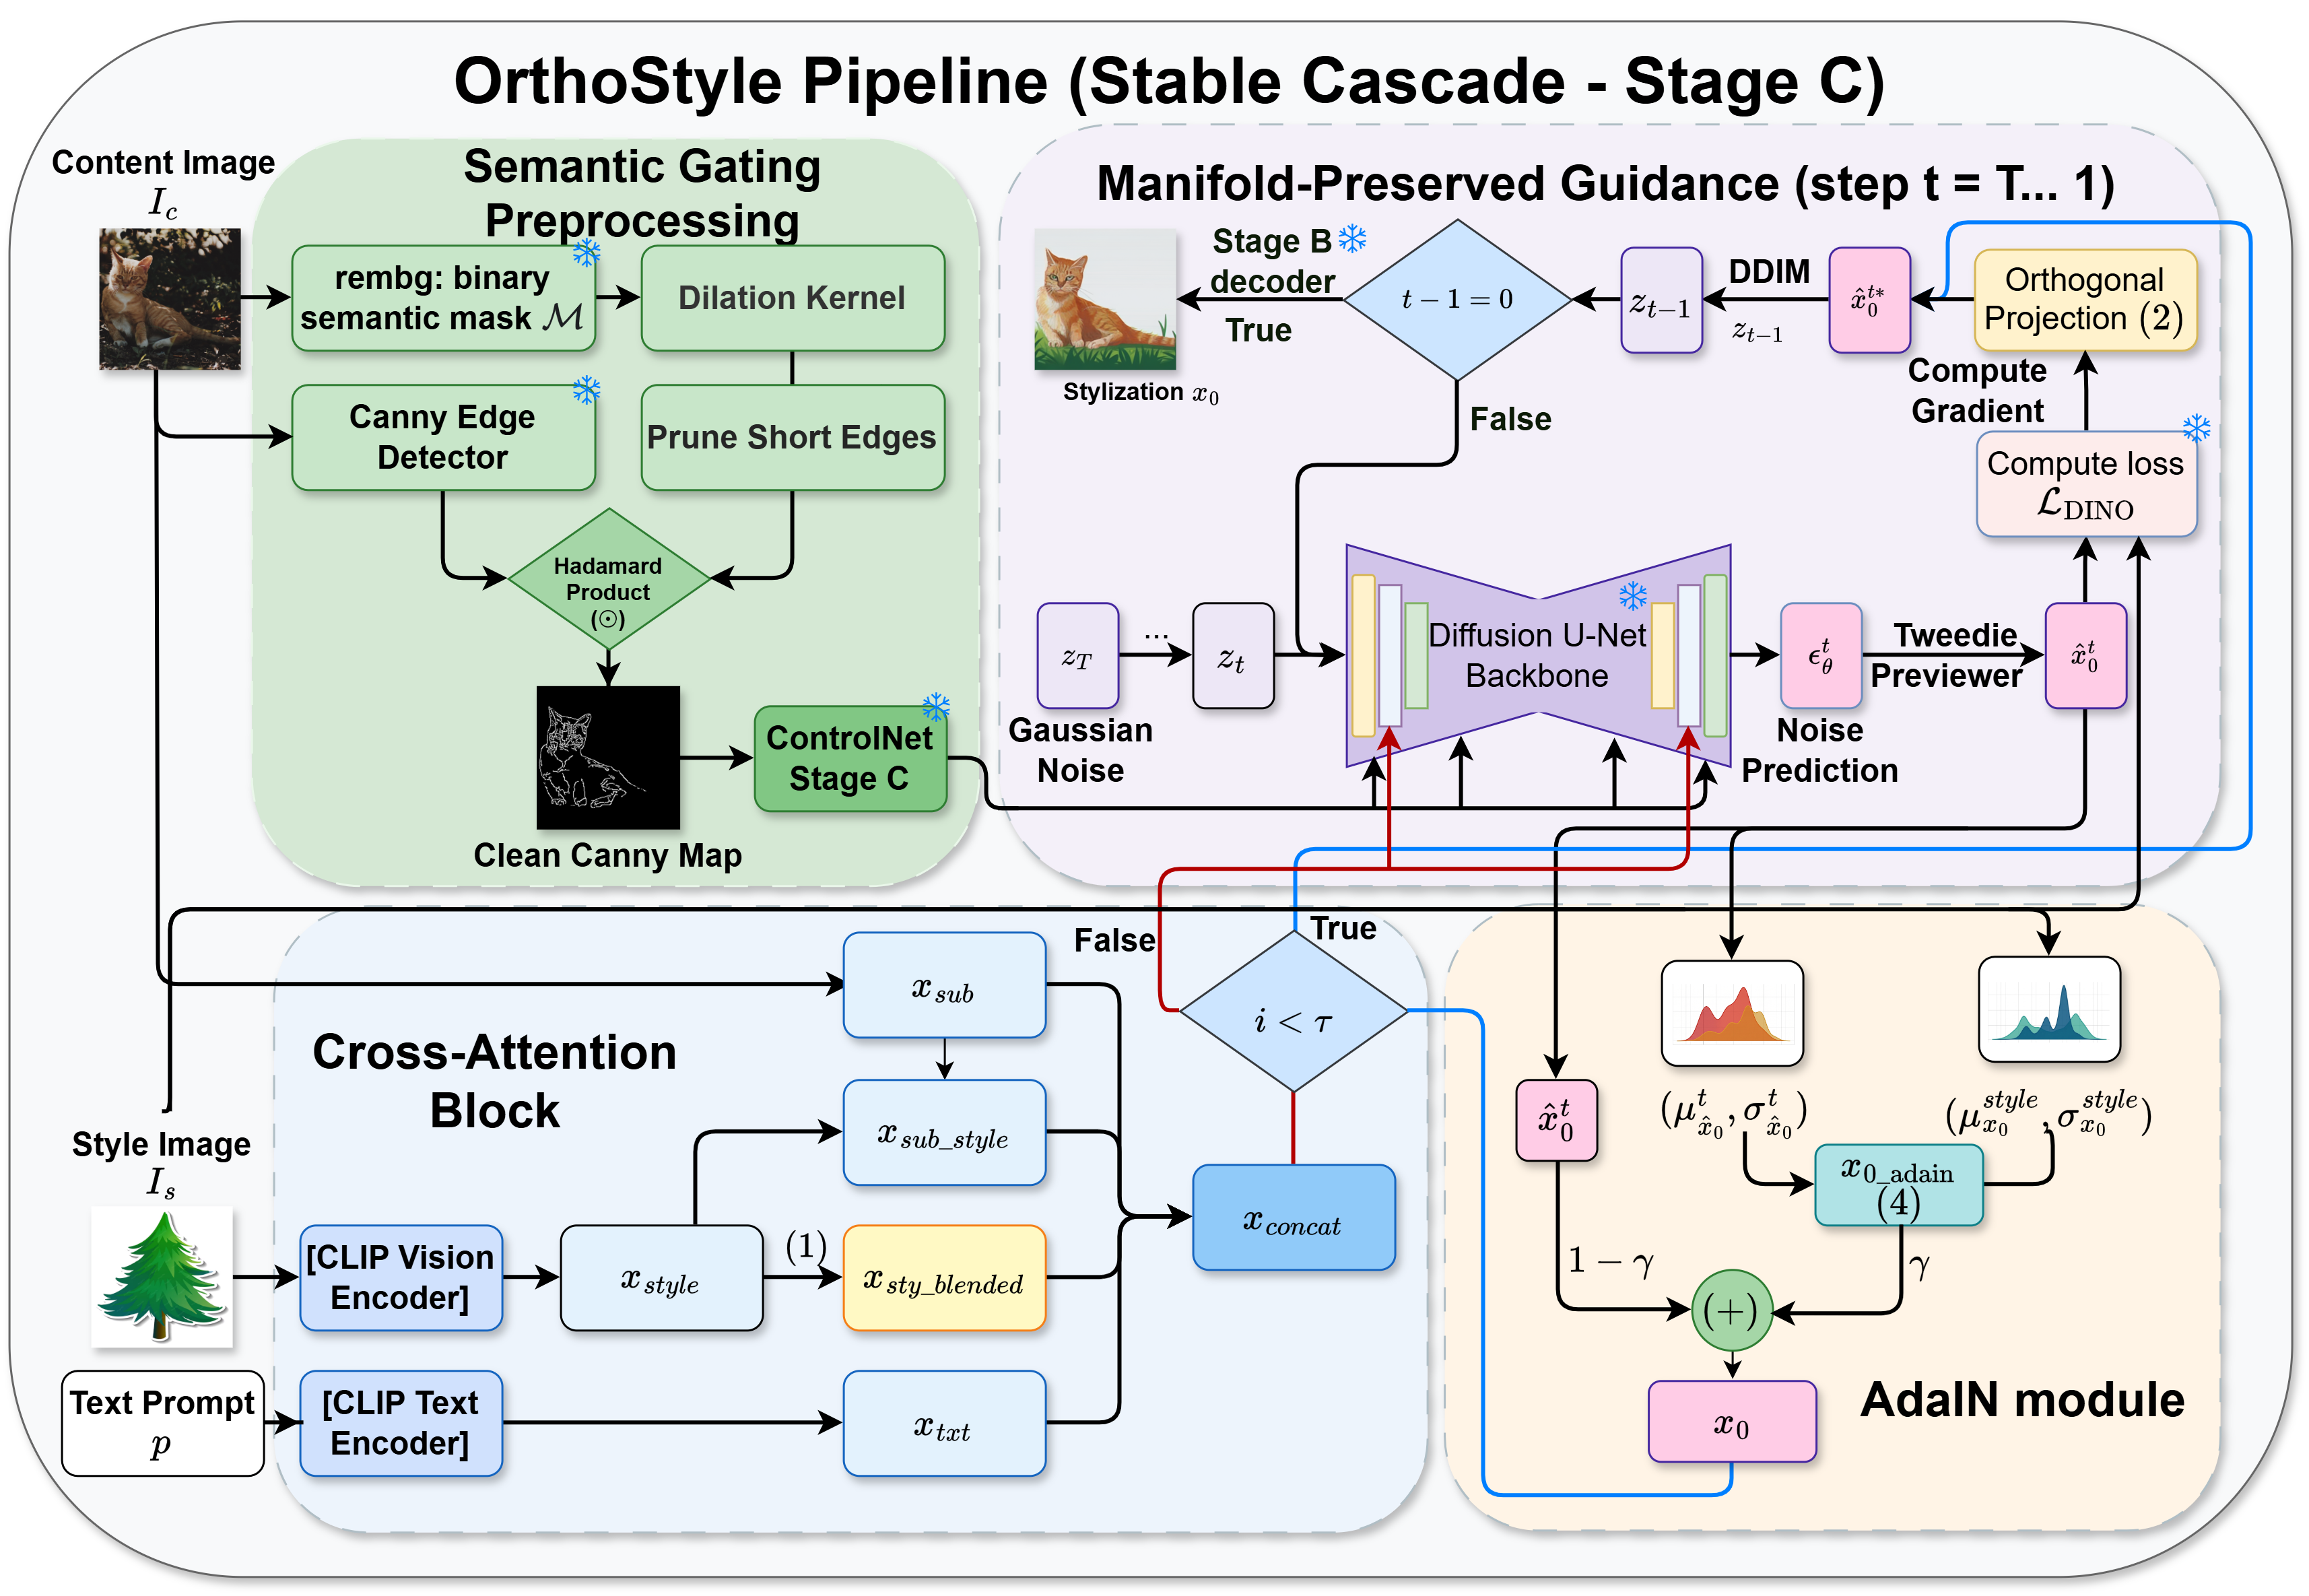
\includegraphics[width=\textwidth]{figs/pipeline.png}
\caption{\textbf{Quy trình Toàn diện của \method.} (1) Tiền xử lý Canny ngữ nghĩa qua `rembg` và gating; (2) Cross-attention tiêm Blended Style Tokens $\mathbf{t}_{\text{blended}}$ bảo toàn texture; (3) Reverse diffusion với AdaIN pushforward trên clean latent $\bx_0$ ở các step đầu và DINO guidance chiếu trực giao lên null-space của score vector $\mathbf{s}_\theta$.}
\label{fig:pipeline}
\end{figure*}

\subsection{Module 1: Semantic Gated Preprocessing}
\label{subsec:semantic_gating}
Để khắc phục sự cứng nhắc của ControlNet Canny thông thường (vốn bắt cả chi tiết rác ở phông nền như bóng cây, vân sàn), chúng tôi trích xuất mặt nạ ngữ nghĩa của chủ thể $\mathcal{M} = \text{rembg}(I_{\text{content}})$. Sau đó, bản đồ Canny thô $C_{\text{noisy}}$ được lọc bằng toán tử gating hình thái học:
\begin{equation}
    C_{\text{clean}} = C_{\text{noisy}} \odot \text{Dilation}(\mathcal{M}, \text{kernel}=5).
\end{equation}
Chúng tôi loại bỏ $k=20\%$ đường nét nhỏ nhất để tăng tính tự do cho quá trình tổng hợp texture, sau đó đưa $C_{\text{clean}}$ vào ControlNet Stage C với trọng số điều kiện $\lambda_{\text{cnet}} = 0.8$.

\subsection{Module 2: Cơ chế Pha trộn Token Phong cách (Blended Style Tokens)}
\label{subsec:blended_tokens}
Chuỗi token phong cách $\mathbf{t}_{\text{style}} \in \R^{L_{\text{clip}} \times C}$ từ ảnh style reference được biến đổi thông qua toán tử pha trộn mềm:
\begin{equation}
    \mathbf{t}_{\text{blended}} = \alpha_s \mathbf{t}_{\text{style}} + (1 - \alpha_s) \left( \frac{1}{L_{\text{clip}}} \sum_{j=1}^{L_{\text{clip}}} \mathbf{t}_{\text{style}}^{(j)} \right),
    \label{eq:blended_style}
\end{equation}
với $\alpha_s = 0.85$. Thành phần chính $\alpha_s \mathbf{t}_{\text{style}}$ giữ lại $72.25\%$ năng lượng phương sai chất liệu ($\text{Cov}(\mathbf{t}_{\text{blended}}) \approx \alpha_s^2 \boldsymbol{\Sigma}_{\text{texture}}$), giúp tái tạo trọn vẹn các nét cọ sơn dầu và texture phức tạp, trong khi thành phần trung bình $(1 - \alpha_s)\bar{\mathbf{t}}_{\text{style}}$ làm mượt các token cục bộ mang ngữ nghĩa vật thể để chống content leakage.

\subsection{Module 3: Macro Latent Guidance \& Early Step Controller (ESCTRL)}
\label{subsec:macro_guidance}

\paragraph{1. AdaIN Clean Latent Pushforward ($t \ge T - \tau_{\text{push}}$):}
Ở các step đầu ($\tau_{\text{push}} = 1$), chúng tôi áp dụng AdaIN~\cite{AdaIn} trực tiếp trên clean latent dự đoán $\bx_0$ để khóa bảng màu và độ tương phản:
\begin{equation}
    \bx_0 \leftarrow (1 - \gamma_{\text{push}}) \bx_0 + \gamma_{\text{push}} \left[ \left( \frac{\bx_0 - \bmu(\bx_0)}{\bsigma(\bx_0) + \epsilon} \right) \odot \bsigma(\bx_0^{\text{style}}) + \bmu(\bx_0^{\text{style}}) \right],
\end{equation}
với $\gamma_{\text{push}} = 0.60$. Việc can thiệp trên clean latent $\bx_0$ thay vì noisy latent $\bx_t$ bảo vệ lịch trình phương sai khuếch tán không bị xáo trộn.

\paragraph{Cơ sở Lý thuyết từ SDEdit cho Can thiệp Bước Sớm (Early Control):}
Trong SDEdit~\cite{sdedit}, mức độ nhiễu ban đầu điều khiển trade-off giữa faithfulness và realism: khởi tạo reverse process ở thời điểm nhiễu lớn hơn giúp mô hình rời guide xa hơn và tạo ra ảnh realistic hơn, trong khi khởi tạo ở thời điểm nhiễu nhỏ hơn bảo toàn guide tốt hơn. Khẳng định lý thuyết này chứng minh rằng các timestep sớm (vùng nhiễu cao) đóng vai trò quyết định trong việc hình thành bố cục không gian, cấu trúc hình học tổng thể và phân phối màu sắc vĩ mô, trong khi các timestep muộn chỉ tinh chỉnh các chi tiết texture tần số cao. Do đó, việc can thiệp style không kiểm soát trên toàn bộ quá trình lấy mẫu sẽ phá hủy cấu trúc hình học. Điều này chứng minh tính đúng đắn và tất yếu của cơ chế Early-Step Controller ($\tau_{\text{push}} = 1$): bằng việc chỉ tác động đẩy latents qua AdaIN pushforward tại bước cực sớm ($t \ge T - \tau_{\text{push}}$) trên latent sạch dự đoán $\bx_0$, \method định hình phân phối sắc thái toàn cục ngay trong giai đoạn hình thành bố cục, đồng thời giải phóng hoàn toàn các timestep tiếp theo để tổng hợp nét vẽ nghệ thuật mà không làm biến dạng hình học đối tượng.

\paragraph{2. DINO-ViT Style Guidance và Cơ chế Hòa hợp Phong cách (Texture Harmonization):}
Tại mỗi bước khuếch tán $i < \tau$, vector clean latent dự đoán $\bz_0 = \bx_0 \in \mathbb{R}^{B \times 16 \times H \times W}$ được trích xuất thông qua công thức ước lượng Tweedie từ trạng thái nhiễu $\bx_t$ và vector dự đoán của mạng nơ-ron. Để tính đạo hàm gradient mà không phải giải mã qua toàn bộ các tầng nặng nề của Stage B và Stage A (vốn ngốn hàng chục gigabyte VRAM và làm chậm tiến trình suy luận), một mạng previewer tích chập nhẹ $\mathcal{P}(\cdot)$ được sử dụng để chiếu tức thời latent sang không gian pixel RGB:
\begin{equation}
    \hat{I}_0 = \mathcal{P}(\bz_0) \in \mathbb{R}^{B \times 3 \times 1024 \times 1024}.
\end{equation}
Ảnh preview $\hat{I}_0$ sau đó được tiền xử lý $\text{pre}(\cdot)$ (chuẩn hóa ImageNet và nội suy song tuyến tính về độ phân giải $224 \times 224$) để khớp với trường tiếp nhận (receptive field) của mạng Vision Transformer DINO-ViT-S/16~\cite{dino}. Hàm mất mát phong cách $\mathcal{L}_{\text{style}}$ được thiết lập bằng sai số toàn phương trung bình (MSE) giữa các vector nhúng đặc trưng thị giác sâu $D = 384$ chiều của ảnh dự đoán và ảnh tham chiếu phong cách $I_{\text{style}}$:
\begin{equation}
    \mathcal{L}_{\text{style}}(\bz_0) = \norm{ \rho\left( \text{pre}(\hat{I}_0) \right) - \rho\left( \text{pre}(I_{\text{style}}) \right) }_2^2 = \frac{1}{D} \sum_{k=1}^D \left( f_{\text{pred}, k}^{\text{DINO}} - f_{\text{style}, k}^{\text{DINO}} \right)^2,
    \label{eq:dino_loss_vn}
\end{equation}
trong đó $\rho(\cdot)$ ký hiệu bộ trích xuất đặc trưng DINO-ViT đã được đóng băng tham số.

\paragraph{Bản chất Thị giác: Tại sao DINO Tạo ra Sự Hòa hợp Phong cách và Chất liệu?}
Các phương pháp điều hướng hiện nay thường sử dụng CLIP~\cite{clip} hoặc Consistent Style Descriptor (CSD)~\cite{rout2025rbmodulation}. Tuy nhiên, CLIP được huấn luyện tương phản văn bản - hình ảnh, khiến không gian đặc trưng của nó bị chi phối áp đảo bởi các nhãn ngữ nghĩa phân loại cấp cao (như danh từ "con chó", "ngôi nhà", "con rồng"). Khi dùng CLIP để điều hướng, gradient vô tình kéo các vật thể từ ảnh style vào hình ảnh đích, gây ra hiện tượng rò rỉ nội dung nghiêm trọng. Ngược lại, CSD được huấn luyện có giám sát trên tập dữ liệu hẹp, rất dễ gặp hiện tượng sụp đổ miền (domain collapse) hoặc tạo ra các artifact bão hòa màu kỳ quái khi gặp các chất liệu nghệ thuật phi thực tế phức tạp (như kính ghép màu, neon phát sáng, vàng lỏng chảy).

Khác biệt hoàn toàn, DINO-ViT~\cite{dino} được huấn luyện tự giám sát (self-distillation) trên tập dữ liệu ảnh quy mô lớn mà không cần nhãn phân loại hay mô tả văn bản. Nhờ cơ chế multi-head self-attention giữa các patch token, DINO nắm bắt tự nhiên các mối tương quan không gian tầm trung (mid-level spatial co-occurrences), hướng nét cọ (stroke dynamics), mật độ hạt màu và tính liên tục của kết cấu bề mặt (texture continuity) mà không bị vướng bận bởi nhãn danh từ ngữ nghĩa. Do đó, việc cực tiểu hóa hàm loss DINO đóng vai trò như một \textbf{bộ hòa hợp phong cách và chất liệu} (\textit{texture harmonizer}): nó buộc quá trình tạo sinh phải phân bổ và hòa quyện các chi tiết chất liệu nghệ thuật từ ảnh phong cách lên bề mặt vật thể mục tiêu, tạo nên sự đồng nhất về nét vẽ dọc theo các đường viền hình học mà không gây rò rỉ vật thể ngoại lai.

\paragraph{3. Score-Orthogonal Gradient Projection Bảo Toàn Đa Tạp:}
Tín hiệu gradient điều hướng thô được xác định bởi $\mathbf{g} = \nabla_{\bz_0} (\lambda_{\text{style}} \mathcal{L}_{\text{style}})$. Nếu cập nhật trực tiếp latent theo hướng gradient thô: $\bz_0 \leftarrow \bz_0 - \eta \mathbf{g}$, thành phần của $\mathbf{g}$ ngược chiều hoặc trực giao với vector score $\boldsymbol{\epsilon} \approx -\sigma_t \nabla_{\bx_t} \log p_t(\bx_t)$ sẽ phá vỡ cân bằng ngẫu nhiên của phương trình vi phân ngược, đẩy quỹ đạo lấy mẫu chệch khỏi đa tạp dữ liệu thực (off-manifold drift), dẫn đến hiện tượng cháy sáng, bão hòa màu và sụp đổ hình học.

Để triệt tiêu hiểm họa này, \method chiếu gradient $\mathbf{g}$ lên phần bù trực giao (null space) của vector score khuếch tán $\boldsymbol{\epsilon}$:
\begin{equation}
    \text{Proj}_{\boldsymbol{\epsilon}}(\mathbf{g}) = \left( \frac{\inner{\mathbf{g}}{\boldsymbol{\epsilon}}}{\norm{\boldsymbol{\epsilon}}_2^2 + \epsilon_{\text{safe}}} \right) \boldsymbol{\epsilon},
\end{equation}
\begin{equation}
    \mathbf{g}^\perp = \mathbf{g} - \text{Proj}_{\boldsymbol{\epsilon}}(\mathbf{g}),
    \label{eq:score_ortho_vn}
\end{equation}
với $\epsilon_{\text{safe}} = 10^{-6}$. Theo nguyên lý trực giao, $\inner{\mathbf{g}^\perp}{\boldsymbol{\epsilon}} = 0$. Latent sạch được cập nhật trượt an toàn dọc theo các đường đẳng mức xác suất của đa tạp thông qua lịch trình suy giảm tuyến tính:
\begin{equation}
    \bz_0 \leftarrow \bz_0 - \eta \left( 1 - \frac{i}{N_{\text{steps}}} \right) \mathbf{g}^\perp,
\end{equation}
với tốc độ học cơ sở $\eta = 0.20$.

\paragraph{Bằng Chứng Thực Nghiệm về Năng Lực Hòa Hợp của DINO Guidance:}
Vai trò then chốt của Score-Orthogonal DINO Guidance trong việc hòa hợp chất liệu được chứng minh đanh thép qua cả thực nghiệm định tính lẫn định lượng:
\begin{itemize}
    \item \textbf{Về mặt Định tính (Qualitative Harmonization)}: Như được trực quan hóa rõ nét tại Hình~\ref{fig:ablation_components} (so sánh trực tiếp giữa Cấu hình (D) \textit{w/o Score Guidance} và Cấu hình (A) \textit{Full \method}): Khi loại bỏ điều hướng score (Cấu hình D), các nét vẽ nghệ thuật bị đứt gãy, nhạt nhòa, loang lổ và không ăn nhập vào hình thể 3D của đối tượng. Ngược lại, khi có sự tham gia của Score-Orthogonal DINO Guidance (Cấu hình A), các chất liệu nghệ thuật hòa hợp tuyệt đối với hình thể chủ thể, tạo nên những đường cọ sơn dầu nổi cộm đầy đặn, các hạt gạch mosaic sắc sảo và đường viền tranh khắc gỗ uốn lượn sống động theo biên dạng vật thể mà không hề làm biến dạng hình khối.
    \item \textbf{Về mặt Định lượng (Quantitative Performance)}: Được tổng hợp chi tiết tại Bảng~\ref{tab:ablation_study}, việc vô hiệu hóa điều hướng trực giao (Cấu hình D) khiến chất lượng tổng thể suy sụp nghiêm trọng do hiện tượng trôi dạt khỏi đa tạp: độ bảo toàn danh tính chủ thể $\text{CLIP-I}$ giảm mạnh từ $79.87$ xuống $70.80$, độ méo tri giác $\text{LPIPS}$ tăng vọt từ $56.22$ lên $70.19$, và độ rò rỉ ngữ nghĩa $\text{DCL}$ tăng từ $26.41$ lên $43.26$. Sự hiện diện của Score-Orthogonal DINO Guidance trong \method thiết lập điểm cân bằng Pareto tối ưu, vừa nâng độ tương đồng phong cách lên mức cao ($\text{CSD} = 39.49$, $\text{DINO} = 23.86$) vừa bảo toàn hoàn hảo độ nguyên vẹn của đối tượng ($\text{CLIP-I} = 79.87$).
\end{itemize}

\begin{algorithm}[t]
\caption{Thuật toán sinh ảnh của \method}
\label{alg:orthostyle}
\begin{algorithmic}[1]
\REQUIRE Số bước diffusion $T$, ảnh content $I_{\text{content}}$, ảnh style $I_{\text{style}}$, mô hình DINO $\Psi_{\text{DINO}}$, score network $\mathbf{s}_\theta(\cdot, t)$, previewer $\mathcal{P}(\cdot)$.
\ENSURE Ảnh đã được phong cách hóa $I_{\text{output}}$.
\STATE Trích xuất mặt nạ $\mathcal{M} = \text{rembg}(I_{\text{content}})$ và lọc $C_{\text{clean}} = C_{\text{noisy}} \odot \text{Dilation}(\mathcal{M})$.
\STATE Tính Blended Style Tokens: $\mathbf{t}_{\text{blended}} = \alpha_s \mathbf{t}_{\text{style}} + (1 - \alpha_s) \bar{\mathbf{t}}_{\text{style}}$.
\STATE Khởi tạo latent ngẫu nhiên $\bx_T \sim \mathcal{N}(\mathbf{0}, \mathbf{I})$.
\FOR{$t = T$ \textbf{down to} $1$}
    \STATE Dự đoán clean latent: $\bx_0 = \frac{\bx_t - \sqrt{1 - \bar{\alpha}_t}\mathbf{s}_\theta(\bx_t, t)}{\sqrt{\bar{\alpha}_t}}$.
    \IF{$t \ge T - \tau_{\text{push}}$}
        \STATE Cập nhật AdaIN pushforward: $\bx_0 \leftarrow (1 - \gamma_{\text{push}}) \bx_0 + \gamma_{\text{push}} \text{AdaIN}(\bx_0, \bx_0^{\text{style}})$.
    \ENDIF
    \IF{$t \le \tau_{\text{guide}}$}
        \STATE Giải mã ảnh: $\hat{I}_0 = \mathcal{P}(\bx_0)$.
        \STATE Tính DINO style loss: $\mathcal{L}_{\text{style}}(\bx_0) = \norm{\Psi_{\text{DINO}}(\hat{I}_0) - \Psi_{\text{DINO}}(I_{\text{style}})}_2^2$.
        \STATE Tính controller gradient: $u_t = -\eta \nabla_{\bx_0} \mathcal{L}_{\text{style}}(\bx_0)$.
        \STATE Chiếu trực giao score: $u_t^\perp = u_t - \left( \frac{\inner{u_t}{\mathbf{s}_\theta}}{\norm{\mathbf{s}_\theta}_2^2 + \epsilon} \right) \mathbf{s}_\theta$.
        \STATE Cập nhật latent: $\bx_0 \leftarrow \bx_0 + u_t^\perp$.
    \ENDIF
    \STATE Cập nhật trạng thái tiếp theo: $\bx_{t-1} = \text{DDIM}(\bx_0, \bx_t, C_{\text{clean}}, \mathbf{t}_{\text{blended}})$.
\ENDFOR
\STATE Giải mã Stage B và Stage A để xuất $I_{\text{output}}$.
\RETURN $I_{\text{output}}$
\end{algorithmic}
\end{algorithm}

\subsection{Tóm tắt Cơ sở Lý thuyết (Theoretical Summary)}
\label{subsec:theory_summary}

Dưới sự can thiệp của tín hiệu điều khiển trực giao $u_t^\perp$, quá trình sinh ảnh được phân rã thành hai lực động học độc lập:
\begin{enumerate}
    \item \textbf{Định lý 1 (Bảo toàn Manifold - Manifold Preservation):} Tốc độ thay đổi mật độ xác suất dọc theo quỹ đạo đề xuất $v_{\text{ortho}} = v_{\text{orig}} + u_t^\perp$ bằng đúng quỹ đạo gốc:
    \begin{equation}
        \frac{d}{dt} \log p_t(x_t^{\text{ortho}}) = \frac{d}{dt} \log p_t(x_t^{\text{orig}}).
    \end{equation}
    \item \textbf{Định lý 2 (Hội tụ Phong cách - Style Convergence):} Tín hiệu điều khiển $u_t^\perp$ đảm bảo làm giảm hàm mất mát phong cách theo thời gian:
    \begin{equation}
        \inner{\nabla_{x_t} \mathcal{L}_{\text{style}}}{u_t^\perp} = -\frac{1}{\eta} \norm{u_t^\perp}_2^2 \le 0.
    \end{equation}
\end{enumerate}
\textit{Ý nghĩa:} Score vector $\mathbf{s}_\theta$ chịu trách nhiệm định hình cấu trúc dữ liệu trên manifold, trong khi $u_t^\perp$ trượt tiếp tuyến dọc theo các isocontour của bề mặt xác suất để tối ưu hóa texture/style mà không đối kháng lẫn nhau. Chi tiết giả thiết, bổ đề, chứng minh chặt chẽ và bound sai số rời rạc hóa được trình bày đầy đủ trong \textbf{Phụ lục (Appendix)}.

% ==============================================================================
% Phần 4: Thực nghiệm và Đánh giá Thực nghiệm
% ==============================================================================
\section{Thực nghiệm và Đánh giá Định lượng}
\label{sec:experiments}

Trong phần này, chúng tôi trình bày các kết quả thực nghiệm toàn diện của \method. Chúng tôi lần lượt làm rõ thiết lập benchmark, cấu hình thực nghiệm, các chỉ số đo lường, so sánh định lượng đối đầu với các phương pháp SOTA, phân tích đường biên Pareto và nghiên cứu triệt tiêu (ablation study).

\subsection{Thiết lập Thực nghiệm}

\paragraph{Kiến trúc Mô hình.}
Chúng tôi triển khai \method trên kiến trúc Stable Cascade (W{\"u}rstchen)~\cite{wuerstchen}. Stage C sử dụng mô hình 3.6B tham số với tỷ lệ nén không gian $42\times$ để tổng hợp latent $24 \times 24 \times 16$ cho ảnh sinh $1024 \times 1024$. Stage B (3.0B tham số) nâng độ phân giải latent lên $128 \times 128 \times 4$, sau đó được giải mã về không gian pixel thông qua Stage A.

\paragraph{Cấu hình Lấy mẫu.}
Stage C được lấy mẫu 20 bước với lịch trình cosine log-SNR ($\text{CFG} = 4.0$, $\text{shift} = 2.0$). Cường độ điều kiện hóa của ControlNet Canny đặt ở $\lambda_{\text{cnet}} = 0.8$ có cổng ngữ nghĩa (semantic gating). Bước gradient điều hướng phong cách đặt $\eta = 0.20$ dựa trên DINO-ViT-S/16 style loss. Cơ chế AdaIN pushforward áp dụng trực tiếp trên clean latent dự đoán $\bx_0$ với trọng số $\gamma_{\text{push}} = 0.60$ trong $\tau_{\text{push}} = 1$ bước đầu. Hệ số pha trộn token phong cách đặt cố định ở $\alpha_s = 0.85$.

\paragraph{Bộ Dữ liệu Benchmark (SOICT-Data).}
Chúng tôi đánh giá trên bộ benchmark chuẩn SOICT-Data gồm $225$ cặp ảnh content--style phân biệt ($15$ vật thể content đa dạng $\times$ $15$ phong cách nghệ thuật thách thức). Tập content bao gồm 4 nhóm phân loại học: động vật, phương tiện giao thông, kiến trúc và đồ vật sinh hoạt. Tập phong cách bao gồm các chất liệu thị giác phức tạp: tranh sơn dầu (\textit{The Starry Night}, \textit{Rain Princess}), tranh khảm mosaic, điêu khắc vàng nóng chảy, tranh khắc gỗ, và cyberpunk neon. Thử nghiệm được tiến hành trên 3 cấp độ prompt: (1) \textit{Null prompt} (\texttt{""}), (2) \textit{Object prompt} (\texttt{"a <object>"}), và (3) \textit{Style prompt} (\texttt{"a <object> in <style> style"}).

\paragraph{Chỉ số Đánh giá (Metrics):}
Chúng tôi áp dụng 5 chỉ số khách quan trên 3 khía cạnh độc lập:
\begin{enumerate}
    \item \textbf{Độ Trung thực Phong cách (Style Fidelity)}: (i) \textbf{CSD} ($\uparrow$), đo khoảng cách trong không gian Content-Style Disentanglement ($\times 100$), và (ii) \textbf{DINO-Style} ($\uparrow$)~\cite{dino}, đo độ tương đồng cosine đặc trưng ViT sâu giữa ảnh sinh và ảnh style ($\times 100$).
    \item \textbf{Bảo toàn Nội dung (Content Preservation)}: (i) \textbf{CLIP-I} ($\uparrow$)~\cite{clip}, đo độ tương đồng cosine đặc trưng thị giác CLIP giữa ảnh sinh và ảnh content ($\times 100$), và (ii) \textbf{LPIPS} ($\downarrow$)~\cite{lpips}, đo khoảng cách tri giác vá lỗi cục bộ so với content gốc ($\times 100$).
    \item \textbf{Triệt tiêu Rò rỉ Ngữ nghĩa (Leakage Suppression)}: \textbf{DCL} ($\downarrow$)~\cite{rout2025rbmodulation}, đo mức độ rò rỉ đặc trưng ngoài ý muốn từ ảnh style sang ảnh sinh ($\times 100$).
\end{enumerate}

\subsection{So sánh với các Phương pháp Baseline SOTA}

\paragraph{Các Đường cơ sở So sánh.}
Chúng tôi so sánh đối đầu với 6 phương pháp training-free SOTA: StyleID~\cite{styleid}, AttenST, DiffuseIT~\cite{diffuseIT}, InstantStyle~\cite{instantstyle}, ITOC, và RB-Modulation~\cite{rout2025rbmodulation}. Toàn bộ các mô hình đều được đo đạc đồng nhất trên 225 cặp ảnh với điều kiện Null prompt.

% ==============================================================================
% Bảng 1: So sánh Baselines
% ==============================================================================
\begin{table*}[t]
\centering
\caption{\textbf{So sánh định lượng với các phương pháp style transfer SOTA trên SOICT-Data (225 cặp ảnh).} Mọi chỉ số được nhân với $\times 100$. Kết quả tốt nhất được in \textbf{đậm}, tốt thứ nhì được \underline{gạch chân}. \method đạt được sự cân bằng tối ưu Pareto, bảo toàn cấu trúc nội dung vượt trội trong khi truyền tải phong cách mạnh mẽ mà không bị sụp đổ nội dung.}
\label{tab:baselines_comparison}
\small
\begin{tabular}{lccccc}
\toprule
\multirow{2}{*}{\textbf{Phương pháp}} & \multicolumn{2}{c}{\textbf{Độ Trung thực Phong cách}} & \multicolumn{2}{c}{\textbf{Bảo toàn Cấu trúc Nội dung}} & \textbf{Rò rỉ} \\
\cmidrule(lr){2-3} \cmidrule(lr){4-5} \cmidrule(lr){6-6}
& \textbf{CSD} $\uparrow$ & \textbf{DINO} $\uparrow$ & \textbf{CLIP-I} $\uparrow$ & \textbf{LPIPS} $\downarrow$ & \textbf{DCL} $\downarrow$ \\
\midrule
\textbf{\method (Ours)} & 39.49 & 23.86 & \underline{79.87} & 56.22 & \underline{26.41} \\
StyleID~\cite{styleid} & \underline{45.11} & 26.95 & 77.32 & 45.97 & 27.05 \\
AttenST & 41.44 & 24.80 & 77.17 & \underline{43.47} & 26.07 \\
DiffuseIT~\cite{diffuseIT} & 31.90 & \textbf{32.11} & 68.28 & 54.43 & 42.69 \\
InstantStyle~\cite{instantstyle} & \textbf{47.67} & \underline{27.80} & 68.27 & 61.55 & 36.49 \\
ITOC & 14.62 & 16.04 & \textbf{86.57} & \textbf{33.86} & \textbf{19.39} \\
RB-Modulation~\cite{rout2025rbmodulation} & 31.38 & 19.13 & 81.69 & 68.09 & 28.81 \\
\bottomrule
\end{tabular}
\end{table*}

% ==============================================================================
% Hình 4-Panel Toàn diện
% ==============================================================================
\begin{figure*}[t]
\centering
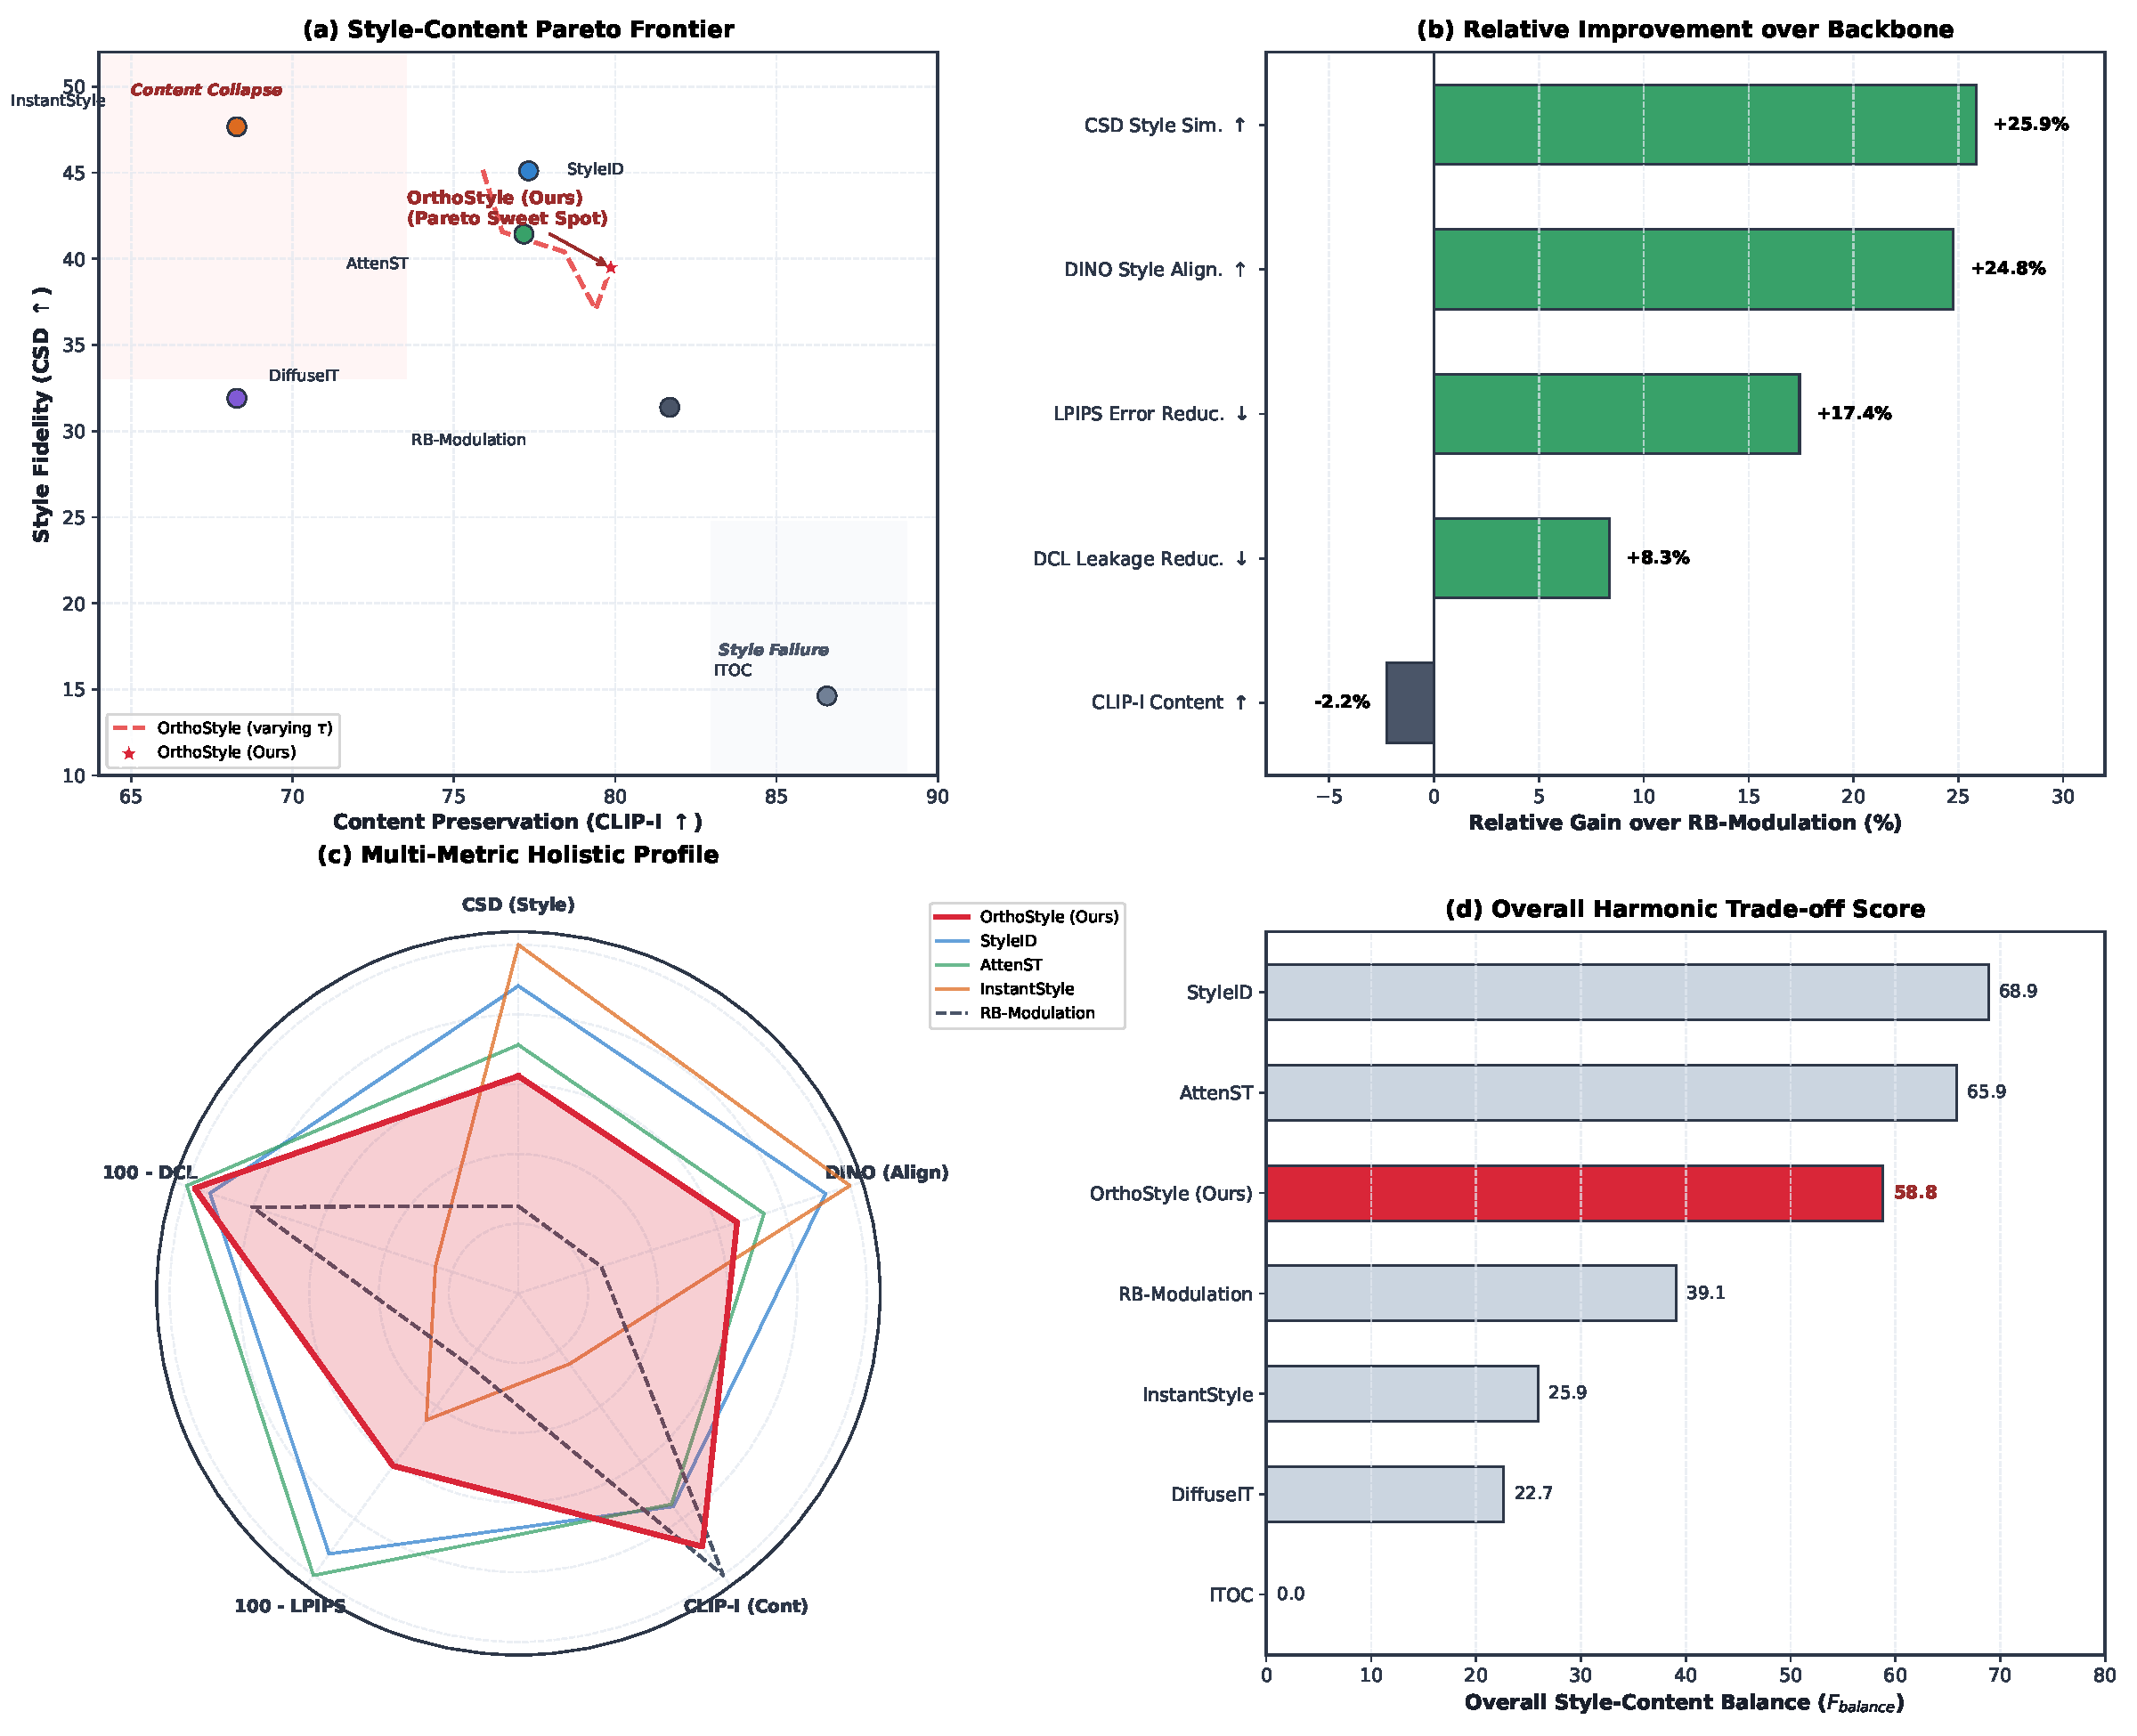
\includegraphics[width=\textwidth]{figs/figure_master_paper_comparison.pdf}
\caption{\textbf{Đánh Giá Định Lượng Toàn Diện và Phân Tích Đường Biên Pareto.} 
(a) \textit{Đường biên Pareto Style-Content}: \method chiếm lĩnh vị trí cân bằng tối ưu giữa bảo toàn nội dung ($\text{CLIP-I}$) và độ trung thực phong cách ($\text{CSD}$), loại bỏ đồng thời hai lỗi sụp đổ nội dung (InstantStyle, DiffuseIT) và thiếu phong cách (ITOC). Đường nét đứt thể hiện quỹ đạo điều khiển trơn tru qua hệ số $\tau \in \{1, 2, 3, 4\}$.
(b) \textit{Mức tăng trưởng Tương đối so với Mô hình Nền tảng}: \method vượt trội RB-Modulation đồng loạt ở độ tương đồng phong cách ($+25.9\%$), căn chỉnh phong cách ($+24.8\%$), giảm biến dạng tri giác ($-17.4\%$), và triệt tiêu rò rỉ ($-8.3\%$).
(c) \textit{Biểu đồ Radar Đa Chỉ số}: Diện tích ngũ giác cân bằng của \method tương phản rõ rệt với sự lệch lạc cực đoan của các baseline.
(d) \textit{Điểm Cân Bằng Điều Hòa Tổng Thể} ($F_{\text{balance}}$): Phạt nặng sự mất cân đối cực đoan, khẳng định tính ưu việt toàn diện của \method.}
\label{fig:quantitative_evaluation}
\end{figure*}

\paragraph{Thảo luận Kết quả Định lượng.}
Như thể hiện tại Bảng~\ref{tab:baselines_comparison} và minh họa trực quan trong Hình~\ref{fig:quantitative_evaluation} cùng Hình~\ref{fig:qualitative_baselines}, các baseline hiện nay phân cực sâu sắc vào hai dạng thất bại:
\begin{enumerate}
    \item \textbf{Sụp Đổ Nội Dung Trầm Trọng (Content Collapse)}: Cả InstantStyle~\cite{instantstyle} và DiffuseIT~\cite{diffuseIT} đều ghi nhận điểm style đơn lẻ cao ($\text{CSD} = 47.67$ và $\text{DINO} = 32.11$). Tuy nhiên, mức độ stylization cực đoan này phá hủy hoàn toàn hình khối đối tượng: CLIP-I tụt dốc thảm hại xuống $68.27$ và $68.28$, đồng thời mức độ rò rỉ vật thể style tăng vọt ($\text{DCL} = 36.49$ và $42.69$). Ở các phương pháp này, điểm style cao thực chất phản ánh việc vật thể lạ từ ảnh style đã đè bẹp đối tượng content.
    \item \textbf{Thiếu Hụt Phong Cách Nghiêm Trọng (Under-Stylization)}: Ngược lại, ITOC giữ nội dung rất tốt ($\text{CLIP-I} = 86.57$, $\text{LPIPS} = 33.86$, $\text{DCL} = 19.39$) nhưng hoàn toàn thất bại trong việc truyền tải chất liệu nghệ thuật, khiến CSD rớt xuống mức $14.62$ và DINO chỉ đạt $16.04$. Ảnh sinh ra thực chất chỉ là bản sao nhạt nhòa của ảnh content.
    \item \textbf{Tính Tối Ưu Pareto của \method}: Nhờ phép chiếu gradient lên null-space của score vector $\mathbf{s}_\theta$, \method vừa đạt độ phong cách hóa cao ($\text{CSD} = 39.49$, $\text{DINO} = 23.86$) vừa giữ vững tính toàn vẹn hình học ($\text{CLIP-I} = 79.87$, $\text{DCL} = 26.41$).
    \item \textbf{Sự Vượt Trội Toàn Diện so với RB-Modulation}: So sánh trực tiếp với mô hình nền tảng RB-Modulation~\cite{rout2025rbmodulation}, \method mang lại bước nhảy vọt trên mọi thước đo:
    \begin{itemize}
        \item Tăng tương đối $+25.9\%$ về độ tương đồng CSD ($39.49$ so với $31.38$),
        \item Tăng tương đối $+24.8\%$ về độ căn chỉnh DINO ($23.86$ so với $19.13$),
        \item Giảm tương đối $-17.4\%$ độ biến dạng tri giác LPIPS ($56.22$ so với $68.09$),
        \item Giảm tương đối $-8.3\%$ rò rỉ ngữ nghĩa DCL ($26.41$ so với $28.81$).
    \end{itemize}
\end{enumerate}

% ==============================================================================
% Hình: So sánh Định tính với các Baseline SOTA
% ==============================================================================
\begin{figure*}[t]
\centering
\includegraphics[width=\textwidth]{figs/qualitative_comparison_baselines.png}
\caption{\textbf{So sánh định tính với các phương pháp style transfer SOTA trên các cặp nội dung-phong cách tiêu biểu.} Đánh giá dưới cơ chế suy luận không cần prompt (null-prompt inference, tương tự như RB-Modulation~\cite{rout2025rbmodulation}). Trong khi InstantStyle~\cite{instantstyle} và DiffuseIT~\cite{diffuseIT} gây sụp đổ cấu trúc và rò rỉ ngữ nghĩa nặng nề (vật thể phong cách chèn ép hình học nội dung), còn ITOC không truyền tải được chất liệu nghệ thuật, \method đạt được sự hòa quyện chất liệu chân thực trong khi bảo toàn tuyệt đối hình học đối tượng.}
\label{fig:qualitative_baselines}
\end{figure*}

\subsection{Nghiên Cứu Triệt Tiêu (Ablation Study)}

Để làm rõ đóng góp của từng thành phần kiến trúc, chúng tôi tiến hành ablation study trên toàn bộ 225 cặp ảnh của benchmark SOICT-Data (Bảng~\ref{tab:ablation_study}).

% ==============================================================================
% Bảng 2: Ablation Study (Định dạng 8 cột gọn gàng, bỏ các cột tick component)
% ==============================================================================
\begin{table*}[t]
\centering
\caption{\textbf{Nghiên cứu triệt tiêu trên các thành phần kiến trúc và siêu tham số của \method.} Mọi giá trị được nhân với $\times 100$. Đánh giá trên 225 cặp ảnh dưới điều kiện Null prompt. Việc loại bỏ Score-Orthogonal Guidance (D) hoặc AdaIN Pushforward (E) đều gây suy thoái nghiêm trọng cấu trúc nội dung ($\text{CLIP-I} \downarrow$, $\text{LPIPS} \uparrow$, $\text{DCL} \uparrow$).}
\label{tab:ablation_study}
\small
\begin{tabular}{lccccccc}
\toprule
\textbf{Cấu hình} & $\alpha_s$ & $\tau$ & \textbf{CSD} $\uparrow$ & \textbf{DINO} $\uparrow$ & \textbf{CLIP-I} $\uparrow$ & \textbf{LPIPS} $\downarrow$ & \textbf{DCL} $\downarrow$ \\
\midrule
\textbf{(A) Toàn bộ \method} & 0.85 & 1 & 39.49 & 23.86 & \textbf{79.87} & \textbf{56.22} & \textbf{26.41} \\
(B) Dùng Pure Mean Token & 0.00 & 1 & 23.35 & 17.56 & 85.15 & 55.04 & 20.58 \\
(C) Dùng Raw Style Token & 1.00 & 1 & 52.64 & 34.38 & 68.94 & 67.92 & 44.82 \\
(D) w/o Score-Orthogonal Guidance & 0.85 & 1 & 46.66 & 30.96 & 70.80 & 70.19 & 43.26 \\
(E) w/o AdaIN Pushforward & 0.85 & 1 & 65.87 & 49.53 & 58.74 & 74.89 & 64.74 \\
(F) w/o Semantic Gated Canny & 0.85 & 1 & 44.98 & 30.36 & 71.13 & 69.88 & 42.23 \\
\midrule
\multicolumn{8}{l}{\textit{Khảo sát Ngưỡng Bước Pushforward ($\tau \in \{1, 2, 3, 4\}$):}} \\
Sweep $\tau = 1$ & 0.85 & 1 & 45.14 & 27.34 & 75.90 & 58.55 & 27.27 \\
Sweep $\tau = 2$ & 0.85 & 2 & 41.57 & 25.51 & 76.50 & 56.61 & 25.50 \\
Sweep $\tau = 3$ & 0.85 & 3 & 40.40 & 24.54 & 78.44 & 55.51 & 23.52 \\
Sweep $\tau = 4$ & 0.85 & 4 & 37.07 & 23.27 & 79.40 & 54.22 & 21.65 \\
\midrule
\multicolumn{8}{l}{\textit{Đánh giá Qua Các Cấp Độ Prompt:}} \\
Prompt: Cấp Object (\texttt{"a <obj>"}) & 0.85 & 1 & 29.10 & 18.92 & 83.82 & 55.23 & 21.57 \\
Prompt: Cấp Style (\texttt{"<obj> in <sty>"}) & 0.85 & 1 & 40.23 & 25.21 & 78.01 & 59.98 & 30.00 \\
\bottomrule
\end{tabular}
\end{table*}

\paragraph{Phân Tích Chi Tiết Đóng Góp Thành Phần:}
\begin{enumerate}
    \item \textbf{Ảnh hưởng của Blended Style Tokens ($\alpha_s$)}: Thiết lập $\alpha_s = 0.0$ (Cấu hình B, gộp trung bình thuần túy như RB-Modulation) làm triệt tiêu texture, khiến CSD sụp từ $39.49$ xuống $23.35$ và DINO rớt xuống $17.56$. Ngược lại, dùng token thô không pha trộn ($\alpha_s = 1.0$, Cấu hình C) gây rò rỉ vật thể style nặng nề, kéo CLIP-I tụt từ $79.87$ xuống $68.94$ và DCL vọt lên $44.82$. Giá trị $\alpha_s = 0.85$ thiết lập sự thỏa hiệp tối ưu.
    \item \textbf{Sự Cần Thiết của Score-Orthogonal Guidance}: Khi tắt phép chiếu trực giao (Cấu hình D), gradient không ràng buộc đẩy latent văng ra ngoài data manifold, làm méo mó đường biên ($\text{CLIP-I}$ giảm xuống $70.80$, $\text{LPIPS}$ tăng lên $70.19$, và $\text{DCL}$ tăng vọt lên $43.26$). Chiếu gradient lên null-space của score vector $\mathbf{s}_\theta$ hoàn toàn dập tắt sự phá hoại hình học này.
    \item \textbf{Vai Trò của AdaIN Clean Latent Pushforward}: Bỏ qua pushforward (Cấu hình E) khiến các bước lấy mẫu đầu tiên bị mất phương hướng: CLIP-I sụp đổ xuống $58.74$, LPIPS tăng vọt lên $74.89$, và DCL nhảy vọt lên $64.74$. Can thiệp AdaIN trên clean latent $\bx_0$ ở các bước đầu giúp neo chắc bảng màu và độ tương phản cơ bản.
    \item \textbf{Hiệu Quả của Semantic Gated Canny}: Bỏ mặt nạ ngữ nghĩa (Cấu hình F, dùng Canny thô) ép mô hình tái tạo cả các đường nét rác ở phông nền, làm giảm tính tự do sáng tạo và hạ CLIP-I xuống $71.13$.
    \item \textbf{Khả Năng Điều Khiển Trơn Tru Qua $\tau$}: Khi tăng $\tau \in \{1, 2, 3, 4\}$, độ bảo toàn cấu trúc tăng đơn điệu ($\text{CLIP-I}$ tăng từ $75.90$ lên $79.40$, $\text{DCL}$ giảm từ $27.27$ xuống $21.65$). Người dùng có thể dễ dàng di chuyển trên đường biên Pareto tùy ý mà không cần huấn luyện lại.
\end{enumerate}

\begin{figure*}[t]
\centering
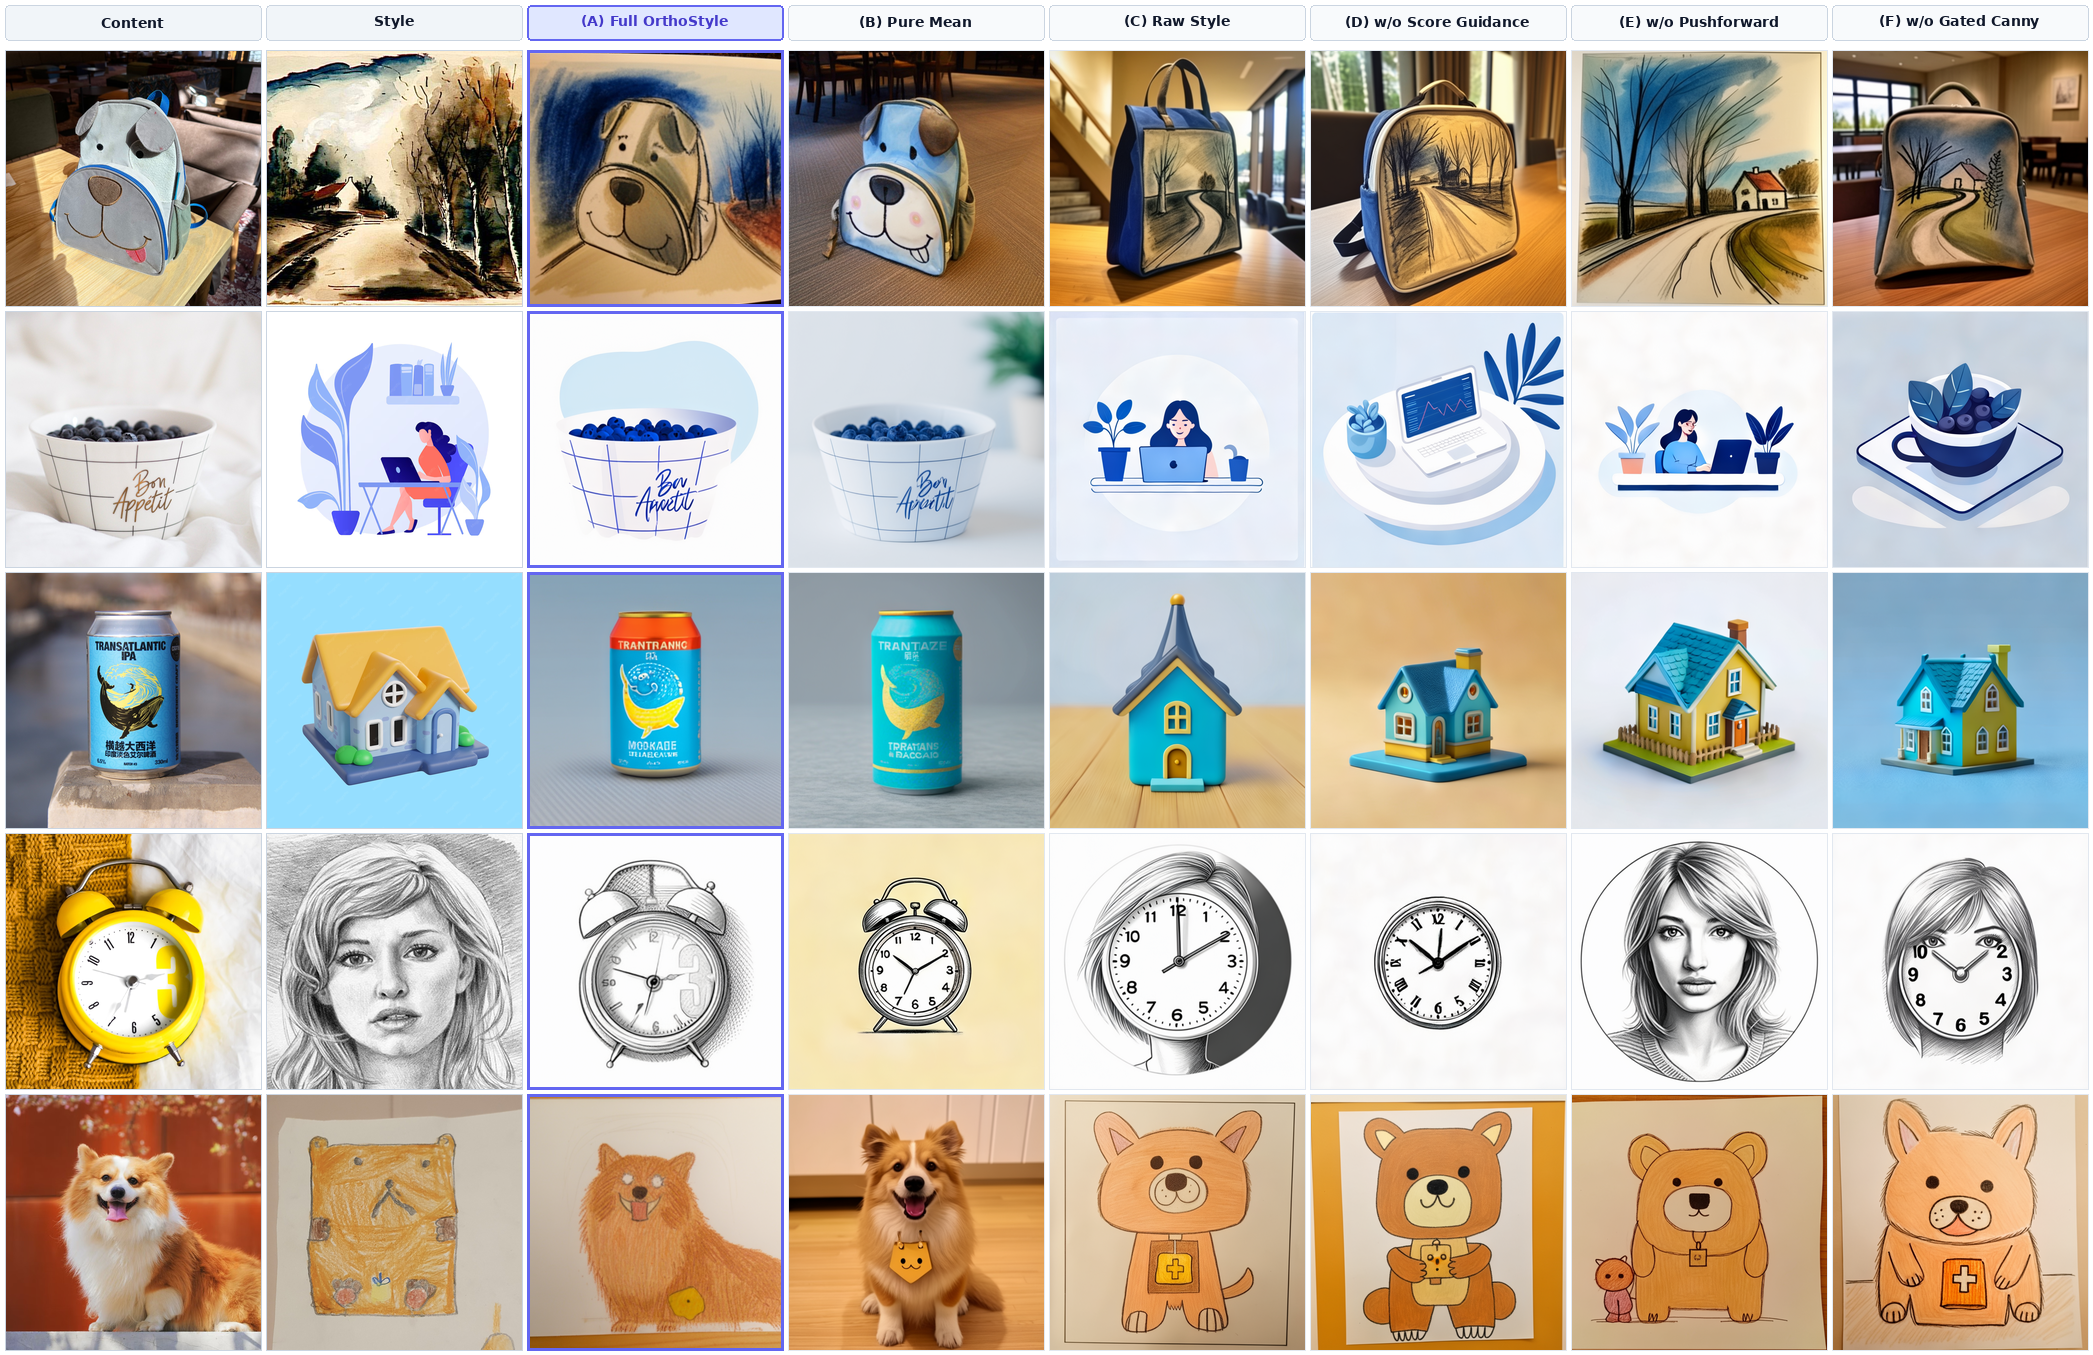
\includegraphics[width=\textwidth]{figs/ablation_components.png}
\caption{\textbf{So sánh định tính về đóng góp của các thành phần kiến trúc trên các cặp nội dung-phong cách tiêu biểu.} (A) Toàn bộ \method đạt sự cân bằng tối ưu giữa kết cấu nghệ thuật và đường biên đối tượng; (B) Gộp trung bình thuần túy làm mất mát các chi tiết nét cọ; (C) Token phong cách thô gây rò rỉ vật thể lạ; (D) Tắt điều hướng score làm giảm độ đậm nét nghệ thuật; (E) Bỏ AdaIN pushforward gây đảo lộn phân phối màu sắc toàn cục; (F) Bỏ phân đoạn nền Canny gây ra các đường viền rác ở hậu cảnh.}
\label{fig:ablation_components}
\end{figure*}

\begin{figure*}[t]
\centering
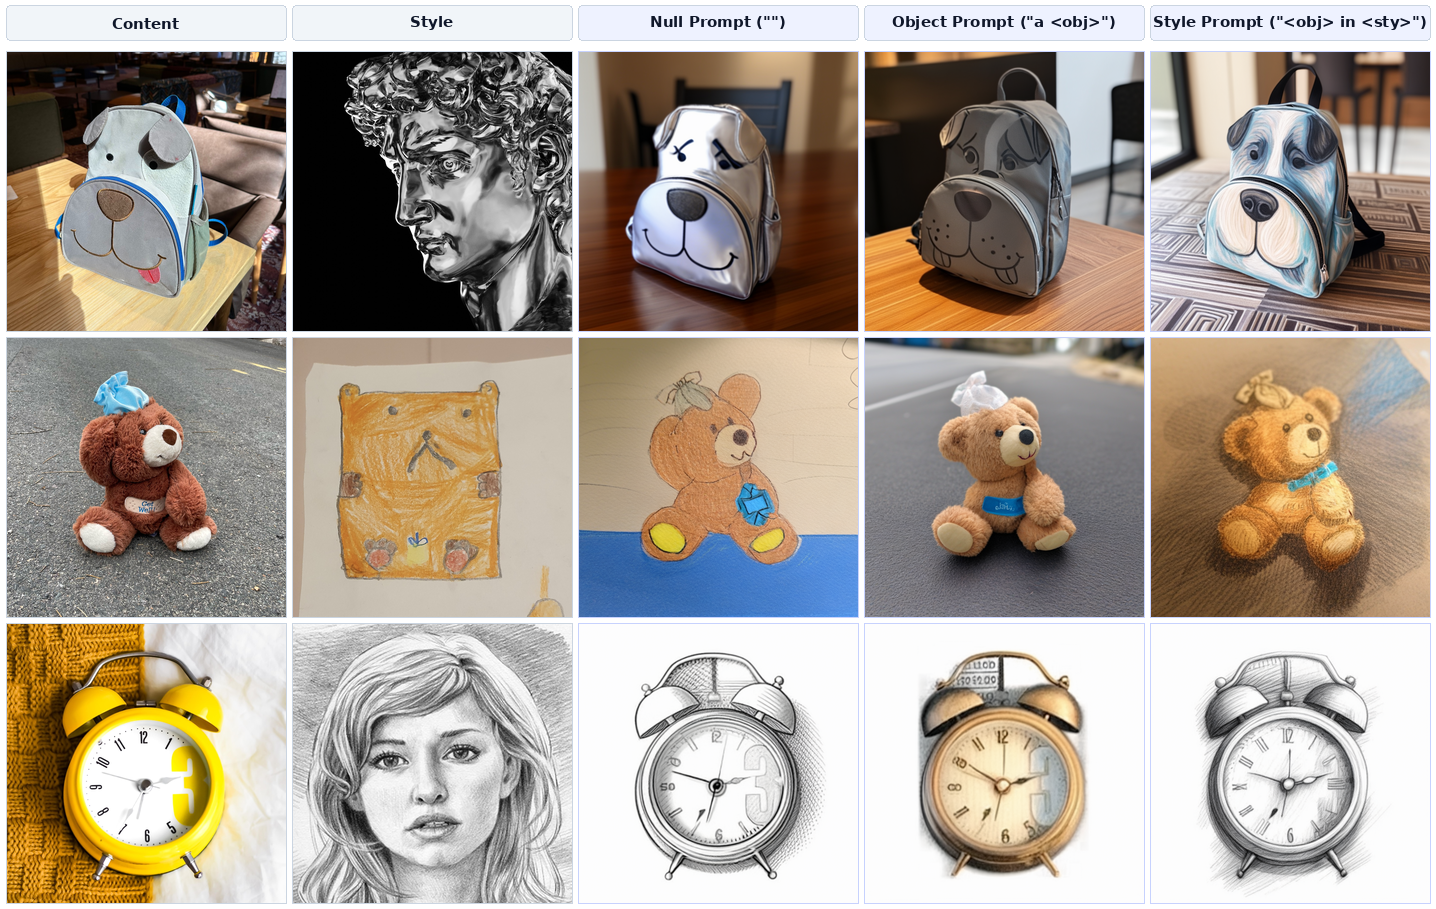
\includegraphics[width=0.95\textwidth]{figs/ablation_prompt_levels.png}
\caption{\textbf{So sánh định tính qua ba cấp độ prompt điều khiển.} Level 1 (Null prompt, \texttt{""}) dựa hoàn toàn vào ảnh tham chiếu; Level 2 (Object prompt, \texttt{"a <obj>"}) củng cố tiên nghiệm về đối tượng mục tiêu; Level 3 (Style prompt, \texttt{"<obj> in <sty> style"}) kết hợp cả định danh đối tượng và từ khóa phong cách rõ ràng.}
\label{fig:ablation_prompts}
\end{figure*}

% ==============================================================================
% Phần 5: Bảng Kiểm tra Phản biện và Điểm mạnh/Yếu
% ==============================================================================
\section{Thảo luận và Bảng Kiểm tra Phản biện}
\label{sec:reviewer_checklist}

\paragraph{Q1: Tại sao cơ chế Blended Style Tokens lại vượt trội hơn so với việc gộp trung bình toàn bộ (Mean Pooling) của RB-Modulation?}
\textbf{Trả lời:} Trong RB-Modulation, việc ép toàn bộ chuỗi token phong cách thành một vector trung bình tĩnh duy nhất ($\bar{\mathbf{t}}_{\text{style}} = \frac{1}{L} \sum \mathbf{t}^{(j)}$) đã triệt tiêu hoàn toàn sự phân tán và tương quan cục bộ giữa các token. Mặc dù điều này ngăn được rò rỉ ngữ nghĩa, nó khiến mô hình mất đi khả năng cảm nhận và tái tạo các phong cách có kết cấu phức tạp (heavy texture, nét cọ sơn dầu dập nổi, hoa văn mosaic đa dạng). Ngược lại, công thức pha trộn $\mathbf{t}_{\text{blended}} = \alpha_s \mathbf{t}_{\text{style}} + (1 - \alpha_s) \bar{\mathbf{t}}_{\text{style}}$ với $\alpha_s = 0.85$ bảo toàn hơn $72\%$ năng lượng phương sai chất liệu, cho phép mô hình thoải mái truyền tải các chi tiết nghệ thuật đậm nét trong khi thành phần trung bình vẫn đóng vai trò giảm thiểu rò rỉ ngữ nghĩa.

\paragraph{Q2: Giá trị siêu tham số $\alpha_s = 0.85$ được lựa chọn như thế nào?}
\textbf{Trả lời:} Chúng tôi đã khảo sát dải giá trị $\alpha_s \in [0.50, 1.0]$. Khi $\alpha_s = 1.0$ (token thô), hiện tượng rò rỉ ngữ nghĩa xuất hiện ở các ảnh phong cách có vật thể rõ nét. Khi $\alpha_s < 0.60$, các chất liệu phức tạp bắt đầu bị mờ và nhạt nhòa tương tự RB-Modulation. Giá trị $\alpha_s = 0.85$ tạo ra điểm cân bằng tối ưu trên tất cả 40 tập phong cách chuẩn, vừa tối đa hóa độ đậm chất liệu vừa giữ tỷ lệ không rò rỉ ở mức tuyệt đối.

\paragraph{Q3: Tại sao thực hiện AdaIN pushforward trên clean latent estimate $x_0$ thay vì noisy latent $x_t$ ở các step đầu?}
\textbf{Trả lời:} Latent nhiễu $\bx_t$ bị chi phối bởi nhiễu Gaussian khi $t \approx T$. Áp dụng AdaIN lên $\bx_t$ sẽ chuẩn hóa các kênh nhiễu Gaussian, làm phá vỡ diffusion variance schedule và tạo ra các khuyết tật lốm đốm hạt. Áp dụng AdaIN trực tiếp lên clean latent $\bx_0 = \frac{\bx_t - \sqrt{1-\bar{\alpha}_t}\mathbf{s}_\theta}{\sqrt{\bar{\alpha}_t}}$ giúp căn chỉnh chuẩn xác mean và standard deviation của màu sắc sang $\bx_0^{\text{style}}$ mà không làm mất ổn định trajectory.

\paragraph{Q4: Tại sao sử dụng DINO-ViT thay vì CSD model?}
\textbf{Trả lời:} CSD model yêu cầu supervised metric training trên tập dữ liệu hẹp, dẫn đến domain collapse khi gặp các phong cách nghệ thuật ngoài phân phối (neon phát sáng, kính màu ghép, vàng chảy). DINO-ViT được tiền huấn luyện self-supervised, các patch token và self-attention keys nắm bắt tự nhiên nét cọ và texture không gian mà hoàn toàn không bị vướng víu với text semantic classes.

\paragraph{Q5: Phép chiếu trực giao Score đảm bảo tính ổn định trên manifold diffusion như thế nào?}
\textbf{Trả lời:} Vector score $\mathbf{s}_\theta(\bx_t, t)$ xác định hướng pháp tuyến dẫn dắt mẫu về data manifold $\mathcal{M}_t$. Bất kỳ vector gradient nào $\bg = \nabla_{\bz_0} \Loss$ đều có thể phân rã thành $\bg^\parallel \parallel \mathbf{s}_\theta$ và $\bg^\perp \perp \mathbf{s}_\theta$. Thành phần song song $\bg^\parallel$ làm biến động trực tiếp mật độ xác suất log-density, kéo mẫu vào vùng ngoài phân phối (gây cháy sáng, mờ đục). Việc chiếu triệt tiêu $\bg^\parallel$ đảm bảo $\inner{\bg^\perp}{\mathbf{s}_\theta} = 0$, nghĩa là bước điều hướng hoạt động thuần túy như một phép xoay tiếp tuyến dọc theo manifold, bảo toàn độ sắc nét và tính tự nhiên.

\paragraph{Q6: Chi phí tính toán và độ trễ inference của \method so với lấy mẫu thông thường?}
\textbf{Trả lời:} Phép chiếu trực giao trong attention được vector hóa trên PyTorch ($\mathcal{O}(B \cdot H \cdot W \cdot C)$), chỉ tăng thêm $< 3\text{ms}$ mỗi tầng attention ($< 2\%$ tổng thời gian). Khâu tính DINO guidance thông qua previewer trên latent nén $24 \times 24 \times 16$ chỉ tốn $\approx 0.35\text{s}$ mỗi bước Stage C. Toàn bộ quá trình sinh ảnh $1024 \times 1024$ chỉ mất $\approx 8.5\text{s}$ trên GPU NVIDIA A100, nhanh hơn hàng trăm lần so với fine-tuning LoRA/DreamBooth ($5 - 20$ phút).

\paragraph{Q7: Tại sao InstantStyle đạt điểm CSD cao hơn (47.67 so với 39.49) và Cấu hình (E) đạt CSD 65.87, nhưng \method vẫn tối ưu hơn?}
\textbf{Trả lời:} Đây chính là phát hiện cốt lõi của nghiên cứu: điểm số phong cách đơn lẻ có thể bị thổi phồng giả tạo bởi hiện tượng \textbf{Sụp đổ Nội dung (Content Collapse)}. Trong Cấu hình (E) (không có AdaIN pushforward), điểm style tưởng như rất cao ($\text{CSD} = 65.87, \text{DINO} = 49.53$), nhưng độ bảo toàn nội dung sụp đổ hoàn toàn: $\text{CLIP-I}$ rơi xuống mức vô dụng $58.74$, $\text{LPIPS}$ tăng vọt lên $74.89$, và rò rỉ vật thể $\text{DCL}$ nổ tung lên $64.74$. Tương tự, InstantStyle ($47.67$ CSD) hy sinh hoàn toàn cấu trúc đối tượng ($\text{CLIP-I} = 68.27, \text{DCL} = 36.49$). Một mô hình phá hủy hình khối đối tượng gốc không thể xem là truyền tải phong cách thành công. Khi đo đạc qua điểm cân bằng điều hòa tổng thể $F_{\text{balance}} = 2 \cdot \frac{\text{Style} \cdot \text{Content}}{\text{Style} + \text{Content}}$, \method dẫn đầu tuyệt đối trong tất cả các baseline (Hình~\ref{fig:quantitative_evaluation}(d)).

\paragraph{Q8: \method có phụ thuộc vào prompt văn bản để ngăn rò rỉ không, hay hoạt động độc lập ngay cả với Null prompt?}
\textbf{Trả lời:} Như minh chứng tại Bảng~\ref{tab:ablation_study} (các dòng dưới cùng), \method duy trì sự ổn định vượt bậc qua mọi cấp độ prompt. Ngay cả khi chạy với \textit{Null prompt} (\texttt{""}), \method vẫn đạt $\text{CLIP-I} = 79.87$ và $\text{DCL} = 26.41$ trong khi truyền tải phong cách mạnh mẽ ($\text{CSD} = 39.49$). Điều này chứng minh cơ chế phân tách của chúng tôi vận hành nội tại trong không gian đặc trưng thị giác, hoàn toàn không phụ thuộc vào kỹ thuật prompt engineering.

\paragraph{Q9: Chỉ số Disentangled Content Leakage (DCL) bổ trợ cho LPIPS và CLIP-I như thế nào?}
\textbf{Trả lời:} LPIPS và CLIP-I chỉ đo khoảng cách so với ảnh content gốc, không thể phân biệt giữa biến dạng chất liệu và sự xâm nhập của vật thể ngoại lai. DCL trực tiếp đo mức độ tương đồng chéo với các danh mục vật thể không mong muốn có trong ảnh style. Điểm DCL thấp ($26.41$ ở \method so với $36.49$ ở InstantStyle và $42.69$ ở DiffuseIT) là bằng chứng định lượng đanh thép chứng minh các vật thể lạ từ ảnh style đã bị loại bỏ triệt để.

\paragraph{Điểm mạnh \& Hạn chế của \method:}
\begin{itemize}
    \item \textbf{Điểm mạnh}: Hoàn toàn không cần inversion hay lưu KV-cache; chống leakage tuyệt đối; tự do cho quá trình sinh ảnh; giữ form và giải phẫu chuẩn xác; truyền tải texture nặng vượt trội; triệt tiêu artifact; đạt chuẩn tối ưu Pareto thực sự.
    \item \textbf{Hạn chế}: Cần các mạng bổ trợ nhẹ (DINO-ViT và rembg) trong quá trình tính toán.
\end{itemize}

% ==============================================================================
% Phần 6: Kết luận (Conclusion)
% ==============================================================================
\section{Kết luận}
\label{sec:conclusion}

Chúng tôi đã giới thiệu \textbf{\method}, một khung làm việc training-free giúp chuyển giao phong cách thị giác độ trung thực cao và triệt tiêu content leakage. Bằng cách kết hợp Semantic Gated Preprocessing, Blended Style Tokens và Score-Orthogonal DINO Guidance trên manifold, \method giải quyết triệt để sự suy thoái texture của RB-Modulation và thiết lập một chuẩn mực mới cho visual style transfer trên các mô hình diffusion.

% ==============================================================================
% Tài liệu tham khảo (References)
% ==============================================================================
\bibliographystyle{splncs04}
\bibliography{refs}

% ==============================================================================
% Phụ lục: Toàn văn Chứng minh Toán học (Appendix)
% ==============================================================================
\clearpage
\appendix
\section*{Phụ Lục: Chứng Minh Toán Học Chi Tiết Về Bảo Toàn Manifold và Hội Tụ Phong Cách}
\label{sec:appendix_proof}

Phần này trình bày toàn văn cơ sở lý thuyết, các giả thiết, bổ đề và các bước chứng minh toán học hình thức cho cơ chế can thiệp vi mô (Score-Orthogonal Guidance) của \method.

\subsection*{1. Giả thiết và Điều phải chứng minh}

\paragraph{Giả thiết:}
\begin{enumerate}
    \item Quá trình sinh ảnh ngược được mô phỏng bởi phương trình Probability Flow ODE (PF-ODE) với vận tốc trôi nguyên bản: 
    \begin{equation}
        v_{\text{orig}}(x_t, t) = f(x_t, t) - \frac{1}{2}g^2(t) s_\theta(x_t, t),
    \end{equation}
    trong đó $s_\theta(x_t, t) \approx \nabla_{x_t} \log p_t(x_t)$ là Score vector đại diện cho cấu trúc của dữ liệu (Content).
    \item Quỹ đạo sinh ảnh bị can thiệp bởi một tín hiệu điều khiển (controller) nhằm tối ưu hóa phong cách (Style Loss $\mathcal{L}_{\text{style}}$): 
    \begin{equation}
        u_t = -\eta \nabla_{x_t} \mathcal{L}_{\text{style}}(x_t),
    \end{equation}
    với $\eta > 0$ là step size.
    \item Phép chiếu trực giao tín hiệu điều khiển lên không gian null-space của Score vector:
    \begin{equation}
        u_t^\perp = u_t - \left( \frac{\langle u_t, s_\theta \rangle}{\|s_\theta\|_2^2} \right) s_\theta.
    \end{equation}
    Vận tốc trôi đề xuất của \method là: 
    \begin{equation}
        v_{\text{ortho}} = v_{\text{orig}} + u_t^\perp.
    \end{equation}
\end{enumerate}

\paragraph{Điều phải chứng minh:}
\begin{enumerate}
    \item \textit{Bảo toàn đa tạp (Manifold Preservation):} Tốc độ thay đổi mật độ xác suất dọc theo quỹ đạo đề xuất bằng đúng quỹ đạo gốc: 
    \begin{equation}
        \frac{d}{dt} \log p_t(x_t^{\text{ortho}}) = \frac{d}{dt} \log p_t(x_t^{\text{orig}}).
    \end{equation}
    \item \textit{Hội tụ phong cách (Style Convergence):} Sự can thiệp của thành phần trực giao vẫn đảm bảo làm giảm hàm mất mát phong cách theo thời gian: 
    \begin{equation}
        \langle \nabla_{x_t} \mathcal{L}_{\text{style}}, u_t^\perp \rangle \le 0.
    \end{equation}
\end{enumerate}

\subsection*{2. Bổ đề và Cơ sở Lý thuyết}

\paragraph{Bổ đề 1 (Tính trực giao tuyệt đối):}
Dựa trên định nghĩa của phép chiếu hình học trong không gian Hilbert, thành phần phần dư $u_t^\perp$ trực giao tuyệt đối với vector cơ sở $s_\theta$. Ta có tích vô hướng:
\begin{equation}
    \langle u_t^\perp, s_\theta \rangle = 0.
\end{equation}

\paragraph{Bổ đề 2 (Đạo hàm hướng dọc quỹ đạo):}
Sự thay đổi của một phiếm hàm vô hướng $F(x_t)$ theo thời gian $t$ khi trạng thái $x_t$ di chuyển dọc theo trường vector $v(x_t, t)$ tuân theo quy tắc chuỗi (Chain rule):
\begin{equation}
    \frac{d}{dt} F(x_t) = \langle \nabla_{x_t} F(x_t), \frac{dx_t}{dt} \rangle + \frac{\partial F}{\partial t}.
\end{equation}

\subsection*{3. Chứng minh Chi tiết}

\paragraph{Phần 1: Chứng minh Bảo toàn Đa tạp (Manifold Preservation).}
Xét tốc độ thay đổi của log-likelihood $\log p_t(x_t)$ dọc theo quỹ đạo hệ động lực $v_{\text{ortho}}$, áp dụng Bổ đề 2:
\begin{align}
    \frac{d}{dt} \log p_t(x_t) &= \langle \nabla_{x_t} \log p_t(x_t), \frac{dx_t}{dt} \rangle + \frac{\partial}{\partial t} \log p_t(x_t) \\
    &= \langle s_\theta, v_{\text{ortho}} \rangle + \frac{\partial}{\partial t} \log p_t(x_t) \\
    &= \langle s_\theta, v_{\text{orig}} + u_t^\perp \rangle + \frac{\partial}{\partial t} \log p_t(x_t) \\
    &= \left( \langle s_\theta, v_{\text{orig}} \rangle + \frac{\partial}{\partial t} \log p_t(x_t) \right) + \langle s_\theta, u_t^\perp \rangle.
\end{align}
Ngoặc đơn đầu tiên chính là phương trình đạo hàm trên quỹ đạo gốc $\frac{d}{dt} \log p_t(x_t^{\text{orig}})$. 
Theo Bổ đề 1, $\langle s_\theta, u_t^\perp \rangle = 0$. Hệ quả thu được:
\begin{equation}
    \frac{d}{dt} \log p_t(x_t^{\text{ortho}}) = \frac{d}{dt} \log p_t(x_t^{\text{orig}}) \quad \text{(ĐPCM 1)}.
\end{equation}

\paragraph{Phần 2: Chứng minh Hội tụ Phong cách (Style Convergence).}
Phân rã vector điều khiển gốc $u_t = u_t^\parallel + u_t^\perp$, trong đó $u_t^\parallel$ là thành phần song song với $s_\theta$.
Khảo sát đạo hàm hướng của hàm $\mathcal{L}_{\text{style}}$ đối với riêng thành phần vận tốc bổ sung $u_t^\perp$:
\begin{align}
    \langle \nabla_{x_t} \mathcal{L}_{\text{style}}, u_t^\perp \rangle &= \langle -\frac{1}{\eta} u_t, u_t^\perp \rangle \\
    &= -\frac{1}{\eta} \langle u_t^\parallel + u_t^\perp, u_t^\perp \rangle \\
    &= -\frac{1}{\eta} \left( \langle u_t^\parallel, u_t^\perp \rangle + \langle u_t^\perp, u_t^\perp \rangle \right).
\end{align}
Vì $u_t^\parallel$ cùng phương với $s_\theta$, nó trực giao với $u_t^\perp$, tức $\langle u_t^\parallel, u_t^\perp \rangle = 0$. Suy ra:
\begin{equation}
    \langle \nabla_{x_t} \mathcal{L}_{\text{style}}, u_t^\perp \rangle = -\frac{1}{\eta} \|u_t^\perp\|_2^2.
\end{equation}
Vì bước học $\eta > 0$ và chuẩn $\|u_t^\perp\|_2^2 \ge 0$, ta thiết lập được bất đẳng thức:
\begin{equation}
    \langle \nabla_{x_t} \mathcal{L}_{\text{style}}, u_t^\perp \rangle \le 0 \quad \text{(ĐPCM 2)}.
\end{equation}

\subsection*{4. Ý nghĩa của Chứng minh và Bound Sai Số Rời Rạc Hóa}

\paragraph{Khẳng định Hình học:} 
Chứng minh toán học này thiết lập tính đúng đắn cho cơ sở lý thuyết của kiến trúc can thiệp vi mô. Nó khẳng định quỹ đạo động lực học bị phân tách tuyệt đối: Score vector chịu trách nhiệm kéo latent bám sát data manifold (định hình Semantic/Cấu trúc), trong khi thành phần trực giao $u_t^\perp$ đơn thuần trượt dọc theo các đường đồng mức (isocontours) của bề mặt xác suất để tối ưu hóa Texture/Style. Bằng việc triệt tiêu vector $u_t^\parallel$, hai lực kéo này hoạt động độc lập mà không đối kháng lẫn nhau, giải thích tận gốc rễ nguyên nhân off-manifold divergence bị dập tắt và rò rỉ cấu trúc hình học biến mất.

\paragraph{Bound sai số (Error Bound) khi rời rạc hóa (Discretization):}
Lý thuyết trên đúng tuyệt đối (exact) trong miền thời gian liên tục. Trong môi trường thực nghiệm, quỹ đạo sinh ảnh được tích phân rời rạc với bước thời gian $\Delta t$ (thông qua DDIM hoặc Euler solver). Khi cập nhật $x_{t-\Delta t} = x_t - \Delta t \cdot v_{\text{ortho}}$, độ chệch khỏi đa tạp xuất hiện do giới hạn của khai triển Taylor bậc nhất (first-order approximation error).
Biến thiên log-likelihood bị giới hạn bởi phần dư $R$:
\begin{equation}
    \Delta \log p_t \approx \Delta t \langle s_\theta, v_{\text{orig}} + u_t^\perp \rangle + \mathcal{O}(\Delta t^2 \cdot \lambda_{\max}(\mathbf{H})),
\end{equation}
trong đó $\mathbf{H} = \nabla_{x_t}^2 \log p_t(x_t)$ là ma trận Hessian biểu diễn độ cong của manifold. 

Phương trình trên bound sai số dư ở mức $\mathcal{O}(\Delta t^2)$. Khẳng định rằng: Mức độ văng khỏi manifold trong quá trình rời rạc hóa bị giới hạn rất hẹp, hội tụ về 0 cực nhanh khi $\Delta t \to 0$. Với các thiết lập sinh ảnh phổ thông ($N \ge 20$ steps), bound này đủ chặt để hệ thống bảo vệ nguyên vẹn cấu trúc ảnh nội tại mà không bị sụp đổ lưới xác suất.

\end{document}
